\documentclass[11pt,letterpaper]{article}
\usepackage[utf8]{inputenc}
\usepackage[T1]{fontenc}
\usepackage{lmodern}
\usepackage[spanish,es-nodecimaldot,es-tabla]{babel}
\usepackage[margin=2.2cm,top=2.4cm,bottom=2.4cm]{geometry}
\usepackage{amsmath,amssymb,amsfonts}
\usepackage{graphicx}
\usepackage{xcolor}
\usepackage{tcolorbox}
\usepackage{array,longtable,tabularx}
\usepackage{enumitem}
\usepackage{setspace}
\usepackage{tikz}
\usetikzlibrary{arrows.meta,positioning,shapes.geometric,calc}
\usepackage{hyperref}

% Paleta institucional Proyecto NÁCAR
\definecolor{nacardark}{HTML}{061A28}
\definecolor{nacarblue}{HTML}{0E4D6C}
\definecolor{nacarcyan}{HTML}{1B8CA6}
\definecolor{nacarlight}{HTML}{EAF6FC}
\definecolor{nacargray}{HTML}{F4F7F9}
\definecolor{nacaralert}{HTML}{8B2635}

\hypersetup{
    colorlinks=true,
    linkcolor=nacarblue,
    urlcolor=nacarcyan,
    citecolor=nacarblue,
    pdftitle={Modelacion Matematica y Computacional de Sistemas de Biofiltracion en el Karst Yucateco - Gemelo Digital Proyecto NACAR},
    pdfauthor={Proyecto NACAR - Ingenieria de Sistemas Ambientales y Gemelo Digital}
}

\setlength{\parskip}{0.45em}
\setlength{\parindent}{0pt}
\emergencystretch=1.8em
\onehalfspacing

\newtcolorbox{destacado}[1][]{
    colback=nacarlight,
    colframe=nacarblue,
    fonttitle=\bfseries,
    coltitle=white,
    colbacktitle=nacarblue,
    boxrule=0.8pt,
    arc=3pt,
    left=8pt,right=8pt,top=6pt,bottom=6pt,
    title={#1}
}

\newtcolorbox{formulabox}[1][]{
    colback=nacargray,
    colframe=nacarcyan,
    fonttitle=\bfseries,
    coltitle=white,
    colbacktitle=nacardark,
    boxrule=0.8pt,
    arc=3pt,
    left=8pt,right=8pt,top=6pt,bottom=6pt,
    title={#1}
}

\begin{document}

% ============================================================================
% PORTADA TÉCNICA
% ============================================================================
\begin{titlepage}
    \centering
    \vspace*{0.2cm}
    {\scshape\Large Proyecto NÁCAR $\cdot$ Bioingeniería Acuática y Modelación Kárstica \par}
    \vspace{0.4cm}
    \rule{\textwidth}{1.5pt}\\[0.35cm]
    {\Huge\bfseries\color{nacardark} Modelación Matemática y Computacional de Sistemas de Biofiltración en el Karst Yucateco \par}
    \vspace{0.3cm}
    {\large\bfseries\color{nacarblue} Especificación Integral del Gemelo Digital (\textit{Digital Twin} -- Versión Offline y Arquitectura Online), Glosario Maestro de Variables, Sistema Explícito de Ecuaciones Acopladas y Flujo de Trabajo Numérico en Módulos Suspendidos \par}
    \vspace{0.25cm}
    \rule{\textwidth}{1.5pt}\\[0.55cm]

    \begin{destacado}[Síntesis Ejecutiva del Documento]
    El presente documento establece de manera rigurosa y autocontenida los fundamentos físicos, químicos, biológicos y computacionales para la construcción del \textbf{Gemelo Digital del Proyecto NÁCAR} en la península de Yucatán. Se desarrolla explícitamente la arquitectura de la \textbf{Versión Offline (Motor Numérico Predictivo y de Dimensionamiento en Python)}, integrando la geometría real de los \textbf{módulos suspendidos de bandejas circulares apiladas (tipo linterna)}, el acoplamiento simbiótico entre bivalvos dulceacuícolas nativos (\textit{Unionidae}), macrófitas regionales (\textit{Typha domingensis} y \textit{Pontederia cordata}), biopelículas bacterianas (marco CWM1 adaptado al trópico) y la coprecipitación kárstica de calcita-fósforo ($\text{CaCO}_3\text{-P}$). Incluye el glosario maestro de variables, la derivación y demostración formal de cada ecuación, el mapa topológico de dependencias funcionales (acopladas vs.\ independientes) y un escenario numérico resuelto paso a paso.
    \end{destacado}

    \vfill
    {\normalsize \textbf{Ubicación Hidrogeológica:} Gran Acuífero Maya, Península de Yucatán ($20^\circ 58'\text{ N}, 89^\circ 37'\text{ W}$)\\[0.15cm]
    \textbf{Arquitectura Numérica:} Modelo de Orden Reducido (ROM 1D/Cuasi-2D Multicapa en Python $\cdot$ SciPy / FastAPI)\\[0.15cm]
    \textbf{Versión del Documento:} Especificación Matemática Consolidada v2.0}
\end{titlepage}

\tableofcontents
\newpage

% ============================================================================
% CAPÍTULO 1
% ============================================================================
\section{Introducción, Justificación y Diagnóstico del Karst Yucateco}

\subsection{El problema como un sistema dinámico complejo}
La biofiltración aplicada a cuerpos de agua artificiales, cenotes o sistemas de tratamiento ecotecnológicos emplazados sobre la plataforma kárstica de la península de Yucatán trasciende la concepción clásica de un reactor estático de lecho fijo. Desde la perspectiva de la ingeniería de sistemas ambientales, un humedal construido o un sistema híbrido de biofiltración con módulos de bivalvos opera como un \textbf{sistema dinámico complejo, abierto, disipativo y altamente no lineal}, donde convergen simultáneamente tres dominios:
\begin{enumerate}[leftmargin=1.5em]
    \item \textbf{Mecánica de fluidos en medios libres, modulares y porosos:} Transporte advectivo, dispersión hidrodinámica, chorros biológicos de bombeo branquial (\textit{exhalant jets}) y resistencia en entramados radiculares.
    \item \textbf{Especiación termodinámica de soluciones carbonatadas:} Equilibrios ácido-base de aguas con dureza cálcica extrema y coprecipitación mineral de ortofosfatos con calcita ($\text{CaCO}_3\text{-P}$).
    \item \textbf{Dinámica poblacional y bioenergética de consorcios multitróficos:} Interacción acoplada entre moluscos bivalvos filtradores en módulos suspendidos, macrófitas emergentes/flotantes y biopelículas bacterianas aerobias, anóxicas y anaerobias.
\end{enumerate}

En el contexto específico del \textbf{Gran Acuífero Maya}, la vulnerabilidad intrínseca de la roca caliza altamente permeable ---caracterizada por redes de fracturas, conductos de disolución y cenotes interconectados que carecen de escorrentía superficial--- amplifica la sensibilidad del ecosistema. Con una recarga anual estimada en $21,813\text{ hm}^3\text{ año}^{-1}$ sobre una superficie de $124,409\text{ km}^2$ (equivalente a una recarga unitaria de $175,336\text{ m}^3\text{ km}^{-2}$), los cuerpos de agua experimentan fluctuaciones drásticas en sus condiciones de frontera.

La presión antropogénica regional ---derivada de la dispersión de excretas líquidas de más de $500$ granjas porcícolas en al menos $13$ municipios críticos, descargas municipales sin tratamiento terciario y actividad turística intensiva en cenotes--- introduce pulsos variables de:
\begin{itemize}[leftmargin=1.5em]
    \item \textbf{Nutrientes:} Nitrógeno amoniacal ($\text{NH}_4^+$), nitratos ($\text{NO}_3^-$ con medias de $205 \pm 260\text{ }\mu\text{M}$ y picos de hasta $413\text{ }\mu\text{mol L}^{-1} \approx 7.90\text{ mg L}^{-1}$) y fósforo reactivo soluble ($\text{PO}_4^{3-}$).
    \item \textbf{Contaminación microbiológica:} Bacterias coliformes fecales ($> 2,400\text{ UFC}/100\text{ mL}$) y $34$ cepas identificadas de \textit{Escherichia coli} multirresistentes a antibióticos.
    \item \textbf{Metales pesados:} Plomo (hasta $80.3\text{ }\mu\text{g L}^{-1}$ en cenotes impactados) y cadmio ($0.1\text{ a }37.9\text{ }\mu\text{g L}^{-1}$).
\end{itemize}

Los diagnósticos hidrogeoquímicos del acuífero demuestran una mineralización carbonatada extrema, con valores regionales de dureza total de $573\text{ a }587\text{ mg L}^{-1}$ como $\text{CaCO}_3$, alcalinidades de $248\text{ a }359\text{ mg L}^{-1}\text{ CaCO}_3$ y concentraciones de bicarbonatos ($\text{HCO}_3^-$) de $302\text{ a }438\text{ mg L}^{-1}$ (Tabla~\ref{tab:cenotes}).

\begin{table}[htbp]
\centering
\caption{Diagnóstico fisicoquímico comparativo en cenotes de Yucatán (condición basal vs.\ pico antropogénico) y extremos regionales documentados para la parametrización de frontera del Gemelo Digital.}
\label{tab:cenotes}
\vspace{0.2cm}
\resizebox{\textwidth}{!}{%
\begin{tabular}{p{4.3cm} c c c c p{3.6cm}}
\hline
\textbf{Parámetro Fisicoquímico} & \textbf{X'batun} & \textbf{X'Canche} & \textbf{Kankirixche} & \textbf{Yokdzonot} & \textbf{Extremos Regionales} \\
 & \scriptsize (Basal / Pico) & \scriptsize (Basal / Pico) & \scriptsize (Basal / Pico) & \scriptsize (Basal / Pico) & \scriptsize (Karst Yucateco) \\
\hline
Temperatura ($^\circ\text{C}$) & $27.4\text{ / }27.7$ & $25.3\text{ / }25.7$ & $27.4\text{ / }27.4$ & $25.2\text{ / }25.4$ & $22.0\text{ a }33.0\,^\circ\text{C}$ \\
pH (unidades) & $6.73\text{ / }6.91$ & $6.91\text{ / }7.08$ & $7.01\text{ / }6.92$ & $7.49\text{ / }7.37$ & $6.73\text{ a }8.10$ \\
Sólidos Disueltos, TDS ($\text{mg L}^{-1}$) & $1440\text{ / }1100$ & $715\text{ / }585$ & $1220\text{ / }1100$ & $676\text{ / }637$ & Media: $865\text{ mg L}^{-1}$ \\
Conductividad ($\mu\text{S cm}^{-1}$) & $2320\text{ / }1900$ & $902\text{ / }912$ & $1960\text{ / }1800$ & $955\text{ / }987$ & Media: $1410\text{ }\mu\text{S cm}^{-1}$ \\
Potencial Redox, ORP ($\text{mV}$) & $-6.1\text{ / }-$ & $-49.6\text{ / }+$ & $-29.6\text{ / }-$ & $-45.8\text{ / }-$ & Reductor: $-60.5\text{ mV}$ \\
Nitratos ($\text{mg L}^{-1}$) & $0.01\text{ / ND}$ & $\text{ND / }7.52$ & $\text{ND / }0.02$ & $\text{ND / }0.05$ & Media: $7.90\text{ mg L}^{-1}$ \\
Dureza / Alcalinidad ($\text{mg L}^{-1}$) & Alta ($\text{Sr, SO}_4^{2-}$) & Dominio $\text{HCO}_3^-$ & Alta ($\text{Sr, K, Cl}^-$) & Reductor ($\text{NH}_4^+$) & Dureza: $573\text{--}587$ \\
\hline
\end{tabular}%
}
\end{table}

\subsection{Limitaciones del enfoque empírico de ``prueba y error'' y meta del Gemelo Digital}
Históricamente, el dimensionamiento de humedales de tratamiento (HSSF y humedales flotantes FTWs) se ha apoyado en reglas heurísticas de ``caja negra'' o ensayos físicos de prueba y error. Este enfoque presenta tres limitaciones insalvables en Yucatán:
\begin{enumerate}[leftmargin=1.5em]
    \item \textbf{Incapacidad de dimensionar la simbiosis almeja--planta:} Si se introducen módulos de bivalvos sin calcular previamente cuánta biomasa vegetal y bacteriana se requiere para absorber sus secreciones metabólicas (amonio $AER$ y mineralización de biodepósitos $ER+PsR$), el propio biofiltro puede acumular amonio tóxico o agotar el oxígeno disuelto ($OCR$).
    \item \textbf{Ceguera ante la colmatación interna (\textit{clogging}):} El monitoreo convencional de entrada/salida oculta la acumulación progresiva de biodepósitos, biopelículas y precipitados de calcita hasta que la conductividad hidráulica cae entre un $45\%$ y un $80\%$, provocando el colapso súbito del sistema.
    \item \textbf{Incapacidad predictiva ante eventos extremos:} Un prototipo calibrado empíricamente no permite predecir la respuesta ante ondas de calor ($>31\text{--}34\,^\circ\text{C}$), choques de turbidez ($>35\text{ mg L}^{-1}$) o picos bacterianos sin construir decenas de réplicas físicas financieramente prohibitivas.
\end{enumerate}

Por consiguiente, la \textbf{Meta del Gemelo Digital del Proyecto NÁCAR} es sustituir el diseño empírico por una plataforma computacional predictiva, adaptativa y automatizada en Python que simule el acoplamiento simultáneo entre la hidrodinámica modular, la bioenergética de los bivalvos, la cinética rizosférica de las macrófitas, el microbioma CWM1 y la química del agua.

\subsection{Alcance de la Fase 1 (Yucatán) y Visión de Escalabilidad Mundial}

\begin{destacado}[Registro de Decisión de Alcance (21 de noviembre de 2026)]
\textbf{Alcance operativo actual:} la Fase 1 del Gemelo Digital se desarrolla, parametriza y valida \textbf{exclusivamente para el karst de Yucatán} y para una \textbf{única especie focal}: \textit{Anodontites trapesialis}. El objetivo inmediato es obtener un modelo presentable y defendible.

\textbf{Visión permanente:} el Proyecto NÁCAR está concebido para \textbf{escalar a nivel mundial}. Toda decisión de diseño de la Fase 1 debe preservar esa posibilidad: ninguna constante regional o biológica se fija dentro de las ecuaciones; todas viven en perfiles intercambiables de región ($\boldsymbol{\Omega}_{\text{región}}$) y de especie ($\boldsymbol{\Theta}_{\text{sp}}$).
\end{destacado}

La estrategia de escalabilidad se apoya en separar las \textbf{leyes de conservación} (balances de masa, transporte, cinéticas de Monod, regla-$\kappa$ DEB), que se suponen generales, de los \textbf{vectores paramétricos locales}, que deben medirse o investigarse para cada nuevo despliegue:
\begin{enumerate}[leftmargin=1.5em,noitemsep]
    \item \textbf{Especie focal (\textit{Anodontites trapesialis}; nombre también referido como \textit{A.\ ciconia}):} se elige por su amplia distribución neotropical, su tasa de aclaramiento reportada ($0.47\text{ a }3.80\text{ L h}^{-1}\text{ ind}^{-1}$) y su producción de nácar. \textbf{Pendientes de verificar antes de presentar:} (a) el estatus taxonómico vigente de \textit{A.\ ciconia} respecto a \textit{A.\ trapesialis} en bases de referencia (p.\ ej.\ MolluscaBase, MUSSEL Project); (b) que la especie sea \textbf{nativa de la cuenca receptora} en la península de Yucatán, condición indispensable bajo la regla del proyecto de no introducir especies exóticas.
    \item \textbf{Perfiles regionales ($\boldsymbol{\Omega}_{\text{región}}$):} el término de coprecipitación calcita-fósforo (Ec.~\ref{eq:sic}) está escrito de forma que se anula cuando $SI_c \le 0$. Esto es un \textbf{mecanismo de diseño}, no un resultado validado: \textbf{no se sabe aún} qué otras regiones del mundo comparten las características hidrogeoquímicas, climáticas y biológicas de Yucatán, ni con qué valores. Caracterizar regiones (dureza, alcalinidad, $SI_c$, temperatura, fotoperiodo, especies nativas disponibles) es una \textbf{meta de investigación de fases posteriores}.
    \item \textbf{Perfiles de especie ($\boldsymbol{\Theta}_{\text{sp}}$):} los parámetros de \textbf{todas} las especies del catálogo ---incluida la especie focal y las especies secundarias--- están \textbf{pendientes de obtenerse} de investigación bibliográfica y/o bioensayos. Los valores de la Tabla~\ref{tab:especies} son semillas provisionales (ver Sección~\ref{sec:estado}).
\end{enumerate}

\newpage
% ============================================================================
% CAPÍTULO 2
% ============================================================================
\section{Arquitectura de Implementación del Gemelo Digital: Versión Offline vs.\ Online}

\subsection{Estrategia Jerárquica y Rol del Motor Numérico Offline}
Como se sintetiza en la Tabla~\ref{tab:complejidad}, una simulación tridimensional CFD completa (Navier-Stokes-Brinkman 3D) tarda entre $12$ y $72\text{ horas}$ de cómputo por escenario, lo que la vuelve inviable como motor interactivo o en tiempo real. Por el contrario, un modelo 0D simple ignora la estratificación vertical entre las raíces flotantes, las columnas de bandejas de almejas y el fondo calcáreo.

\begin{table}[htbp]
\centering
\caption{Compromiso (\textit{trade-off}) entre resolución física, tiempo de cómputo y viabilidad operativa para el Gemelo Digital.}
\label{tab:complejidad}
\vspace{0.2cm}
\resizebox{\textwidth}{!}{%
\begin{tabular}{p{3.4cm} p{3.8cm} c p{4.6cm} p{4.2cm}}
\hline
\textbf{Nivel de Modelo} & \textbf{Base Matemática} & \textbf{Tiempo (30 días)} & \textbf{Aplicación en NÁCAR} & \textbf{Viabilidad Gemelo Digital} \\
\hline
\textbf{0D (CSTR Simple)} & Sistema de EDOs en $1$ volumen de control & $< 0.05\text{ s}$ & Balances estequiométricos rápidos y dimensionamiento preliminar de biomasa & Alta en velocidad; útil para despejes analíticos globales ($m^*$). \\
\hline
\textbf{1D/Cuasi-2D Multicapa (ROM)} & Red de $N \times 3$ celdas acopladas (EDOs rígidas) & $\mathbf{0.5\text{ a }3.0\text{ s}}$ & \textbf{Motor principal del Gemelo Digital (Offline y Online)}; predicción temporal y control & \textbf{Óptima:} Resuelve gradientes axiales y los 3 estratos verticales casi al instante. \\
\hline
\textbf{2D Reactivo (FiPy)} & EDPs elípticas/parabólicas (Richards + CWM1) & $10\text{ a }90\text{ min}$ & Evaluación fuera de línea de frentes espaciales de colmatación $K(x,z,t)$ & Media-Baja directa; uso de calibración en laboratorio. \\
\hline
\textbf{3D CFD Completo} & Navier-Stokes 3D + transporte reactivo & $12\text{ a }72\text{ h}$ & Diseño hidrodinámico puntual de geometría de bandejas & Inviable en línea; destilado en el factor $\eta_{\text{mod}}$. \\
\hline
\end{tabular}%
}
\end{table}

La implementación del Gemelo Digital se divide estratégicamente en dos versiones complementarias que comparten el mismo núcleo matemático:

\begin{enumerate}[leftmargin=1.5em]
    \item \textbf{Versión Offline (\textit{In-Silico Design \& Predictive Engine} -- Etapa Actual):}
    Es el motor de backend autónomo en Python (\texttt{scipy.integrate.solve\_ivp} con integradores implícitos \texttt{Radau}/\texttt{BDF} para ecuaciones rígidas). No requiere que los sensores IoT estén transmitiendo en vivo; en su lugar, recibe del usuario:
    \begin{itemize}
        \item \textbf{Datos ``sacables a vista'' (configuración física):} Volumen y dimensiones de la figura de agua, número de módulos tipo linterna ($M_{\text{mod}}$), número de pisos por módulo ($K_{\text{pisos}}$), diámetro de bandeja ($D_b$), distancia entre pisos ($h_{\text{piso}}$), cantidad de almejas ($n_b$) o distancia entre ellas ($d_{\text{almejas}}$), longitud media de concha ($L$) y área o biomasa de macrófitas ($A_{\text{mac}}$ o $m$).
        \item \textbf{Condiciones iniciales del agua ($t=0$):} Concentración inicial de bacterias patógenas ($X_{\text{pat}}(0)$), turbidez o sólidos suspendidos ($TSS(0)$), amonio ($S_{NH}(0)$), nitratos ($S_{NO}(0)$), fosfatos ($S_{PO4}(0)$), oxígeno disuelto ($S_O(0)$), temperatura ($T$) y $\text{pH}$. Si algún parámetro geoquímico avanzado no se mide, el módulo \textit{Soft-Sensor Karst Mapper} asigna automáticamente la línea base del acuífero yucateco (Tabla~\ref{tab:cenotes}).
    \end{itemize}
    Con estas entradas, la Versión Offline calcula instantáneamente: (a) la \textbf{biomasa crítica de plantas $m^*$} necesaria para neutralizar las secreciones de las $n$ almejas, (b) las \textbf{curvas completas de evolución temporal} de calidad del agua hora por hora, (c) el \textbf{tiempo exacto en horas ($t_{\text{meta}}$)} para bajar las bacterias y turbidez al umbral deseado, y (d) el \textbf{calendario de mantenimiento por colmatación} de las bandejas.

    \item \textbf{Versión Online (\textit{Living Digital Twin} con Sensores IoT -- Etapa de Campo):}
    Conecta el motor Offline a un pipeline de telemetría \texttt{MQTT} $\to$ \texttt{InfluxDB} $\to$ \texttt{FilterPy (EnKF)} $\to$ \texttt{FastAPI}. Cada $5\text{ a }15\text{ minutos}$, las sondas multiparamétricas en el humedal envían lecturas reales de $T, \text{pH}, S_O, \text{Turbidez NTU}, \text{Conductividad}, \text{ORP}, S_{NH}$ y $S_{NO}$. El Filtro de Kalman compara la predicción del modelo contra el sensor y corrige en vivo el estado interno del reactor.
\end{enumerate}

\newpage
% ============================================================================
% CAPÍTULO 3
% ============================================================================
\section{Conceptualización Física del Módulo de Almejas y Glosario Maestro de Variables}

\subsection{Anatomía Geométrica e Hidrodinámica de los Módulos Suspendidos Tipo ``Linterna''}
A diferencia de la siembra directa sobre el fango bentónico ---donde los bivalvos quedan expuestos a hipoxia severa, enterramiento por sedimentos y dificultad de manejo operativo---, el Proyecto NÁCAR implementa \textbf{módulos suspendidos de bandejas circulares apiladas verticalmente (columnas tipo linterna)}, tal como se ilustra en la Figura~\ref{fig:modulo}.

\begin{figure}[htbp]
    \centering
    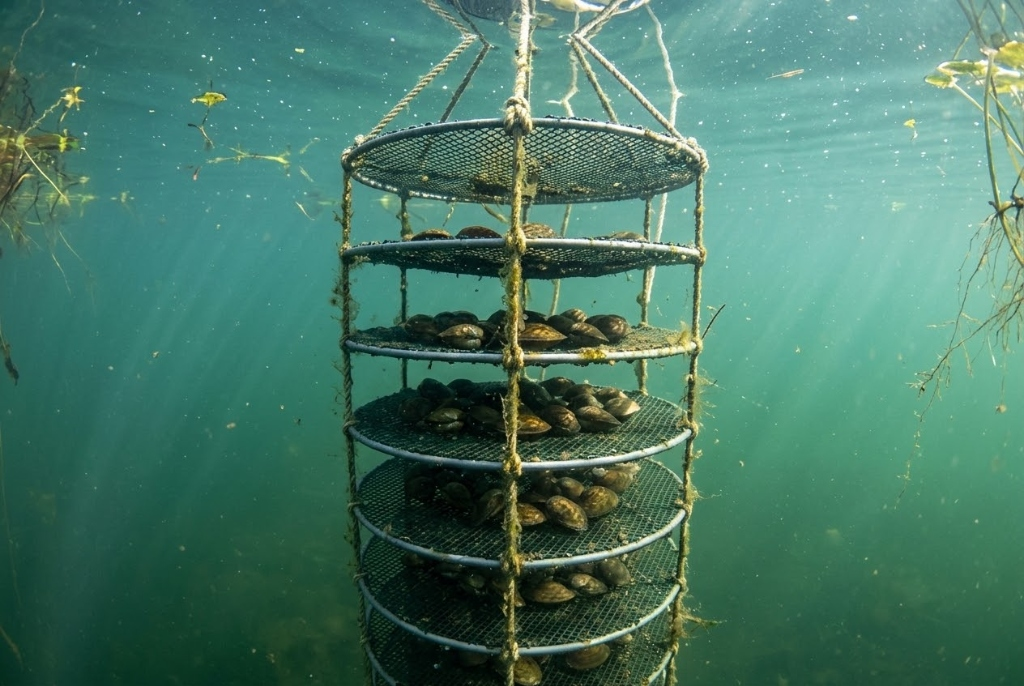
\includegraphics[width=0.72\textwidth]{modulo_linterna_almejas.jpg}
    \caption{Configuración física de referencia del módulo de biofiltración del Proyecto NÁCAR: columna cilíndrica suspendida tipo linterna compuesta por $K_{\text{pisos}}$ bandejas circulares de malla polimérica donde se distribuyen los bivalvos filtradores ($n_b$ individuos por piso separados a distancia $d_{\text{almejas}}$), flanqueada lateral y superiormente por la rizosfera sumergida de macrófitas acuáticas.}
    \label{fig:modulo}
\end{figure}

Desde el punto de vista de la física del transporte y del balance de masa, esta geometría modular introduce cuatro fenómenos determinantes que nuestras ecuaciones capturan explícitamente:
\begin{enumerate}[leftmargin=1.5em]
    \item \textbf{Distribución en discos por piso ($D_b, n_b, d_{\text{almejas}}$):} Cada módulo ($M_{\text{mod}}$) posee $K_{\text{pisos}}$ pisos circulares de diámetro $D_b$, separados verticalmente por $h_{\text{piso}}$. Sobre cada bandeja se alojan $n_b$ bivalvos nativos (familia \textit{Unionidae}, ej.\ \textit{Anodontites trapesialis}), dando una población total $n = M_{\text{mod}} \cdot K_{\text{pisos}} \cdot n_b$.
    \item \textbf{Competencia hidrodinámica horizontal ($\eta_{\text{horiz}}$):} Si la distancia horizontal entre almejas vecinas ($d_{\text{almejas}}$) dentro del mismo disco es menor que dos veces el radio de influencia del sifón inhalante ($\ell_{\text{sifón}}$), los individuos compiten por la misma parcela de agua y re-filtran líquido ya procesado.
    \item \textbf{Acoplamiento vertical entre pisos apilados ($\eta_{\text{vert}}$):} Los chorros exhalantes verticales (\textit{jets}) del piso inferior ascienden hacia el piso superior a menos que la separación vertical $h_{\text{piso}}$ y la corriente cruzada horizontal $v_x$ deflecten la pluma fuera de la columna.
    \item \textbf{Interacción directa con la rizosfera periférica ($m, A_{\text{mac}}$):} Las raíces sumergidas de \textit{Typha domingensis} y \textit{Pontederia cordata} que rodean las linternas interceptan directamente la pluma de amonio ($AER$) excretada por las almejas y suministran oxígeno radicular hacia la columna intermedia.
\end{enumerate}

\subsection{Glosario Maestro de Términos, Variables y Parámetros de las Ecuaciones}
La Tabla~\ref{tab:glosario} define exhaustivamente cada símbolo empleado en las ecuaciones del Gemelo Digital, su unidad física, su categoría operativa y su rango de valores en el karst yucateco.

{\small
\begin{longtable}{p{1.85cm} p{5.95cm} p{2.15cm} p{2.15cm} p{2.55cm}}
\caption{Glosario Maestro de Variables y Parámetros del Gemelo Digital del Proyecto NÁCAR.} \label{tab:glosario} \\
\hline
\textbf{Símbolo} & \textbf{Nombre y Significado Físico} & \textbf{Unidades} & \textbf{Categoría} & \textbf{Rango / Valor Karst} \\
\hline
\endfirsthead
\multicolumn{5}{c}{{\bfseries \tablename\ \thetable{} -- Continuación del Glosario Maestro}} \\
\hline
\textbf{Símbolo} & \textbf{Nombre y Significado Físico} & \textbf{Unidades} & \textbf{Categoría} & \textbf{Rango / Valor Karst} \\
\hline
\endhead
\hline \multicolumn{5}{r}{{Continúa en la siguiente página...}} \\ \hline
\endfoot
\hline
\endlastfoot

\multicolumn{5}{l}{\textbf{A. Variables Geométricas y de Diseño Físico (``Sacables a Vista'')}} \\
\hline
$V$ & Volumen total efectivo de agua del humedal o celda de control & $\text{L}$ (o $\text{m}^3$) & Entrada a vista & $5,000\text{--}100,000\text{ L}$ \\
$A_{\text{hum}}$ & Área superficial del espejo de agua (``figura de agua'') & $\text{m}^2$ & Entrada a vista & $5.0\text{--}150.0\text{ m}^2$ \\
$H$ & Profundidad media de la columna de agua ($V / (1000\,A_{\text{hum}})$) & $\text{m}$ & Entrada a vista & $0.8\text{--}2.0\text{ m}$ \\
$M_{\text{mod}}$ & Número de columnas modulares tipo linterna sumergidas & $\text{módulos}$ & Entrada a vista & $1\text{--}20\text{ módulos}$ \\
$K_{\text{pisos}}$ & Número de bandejas circulares apiladas por módulo & $\text{pisos/mód}$ & Entrada a vista & $5\text{--}7\text{ pisos}$ \\
$D_b$ & Diámetro de cada bandeja circular de malla & $\text{cm}$ & Entrada a vista & $45\text{--}60\text{ cm}$ \\
$h_{\text{piso}}$ & Separación vertical entre bandeja y bandeja en la linterna & $\text{cm}$ & Entrada a vista & $15\text{--}25\text{ cm}$ \\
$n_b$ & Número de bivalvos colocados en cada bandeja circular & $\text{ind/piso}$ & Entrada a vista & $15\text{--}35\text{ ind}$ \\
$n$ & Cantidad total de bivalvos en el sistema ($M_{\text{mod}}\cdot K_{\text{pisos}}\cdot n_b$) & $\text{ind}$ & Entrada a vista & $50\text{--}2,500\text{ ind}$ \\
$d_{\text{almejas}}$ & Distancia media centro-a-centro entre almejas vecinas en bandeja & $\text{cm}$ & Entrada / Calc. & $3.5\text{--}14.0\text{ cm}$ \\
$L$ & Longitud anteroposterior media de la concha del bivalvo & $\text{mm}$ & Entrada a vista & $45\text{--}85\text{ mm}$ \\
$A_{\text{mac}}$ & Área superficial cubierta por macrófitas flotantes/emergentes & $\text{m}^2$ & Entrada a vista & $1.0\text{--}50.0\text{ m}^2$ \\
$m$ (o $B_{\text{mac}}$) & Biomasa seca activa de raíces (rizosfera sumergida) de macrófitas & $\text{kg MS}$ & Entrada / Calc. & $0.80\text{ kg MS/m}^2$ \\
$v_x$ & Velocidad horizontal media de circulación del agua a través de la linterna & $\text{cm}\cdot\text{s}^{-1}$ & Hidrodinámica & $0.5\text{--}5.0\text{ cm/s}$ \\
$Q_{\text{in}}$ & Caudal volumétrico de entrada externa al humedal ($0$ en lote) & $\text{L}\cdot\text{h}^{-1}$ & Hidrodinámica & $0\text{--}2,000\text{ L/h}$ \\
\hline

\multicolumn{5}{l}{\textbf{B. Variables de Estado Dinámicas y Lecturas de Sensores IoT}} \\
\hline
$T$ & Temperatura del agua en la columna intermedia & $^\circ\text{C}$ & Sensor IoT & $22.0\text{--}34.0\,^\circ\text{C}$ \\
$\text{pH}$ & Potencial de hidrógeno de la solución kárstica & $\text{unid. pH}$ & Sensor IoT & $6.73\text{--}8.10$ \\
$S_O$ & Concentración de Oxígeno Disuelto ($\text{OD}$) en el agua & $\text{mg O}_2\cdot\text{L}^{-1}$ & Estado / IoT & $2.0\text{--}8.2\text{ mg/L}$ \\
$TSS$ & Sólidos Suspendidos Totales / Materia Particulada ($TPM$, de NTU) & $\text{mg MS}\cdot\text{L}^{-1}$ & Estado / IoT & $3.0\text{--}45.0\text{ mg/L}$ \\
$X_{\text{pat}}$ & Concentración de bacterias patógenas (\textit{E. coli} / Coliformes fecales) & $\text{UFC}/100\text{mL}$ & Variable Estado & $0\text{--}5,000\text{ UFC}$ \\
$S_{NH}$ & Nitrógeno amoniacal total disuelto ($\text{NH}_4^+\text{-N} + \text{NH}_3\text{-N}$) & $\text{mg N}\cdot\text{L}^{-1}$ & Estado / IoT & $0.05\text{--}8.0\text{ mg/L}$ \\
$S_{NO}$ & Nitrógeno oxidado total ($\text{NO}_3^-\text{-N} + \text{NO}_2^-\text{-N}$) & $\text{mg N}\cdot\text{L}^{-1}$ & Estado / IoT & $0.05\text{--}7.90\text{ mg/L}$ \\
$S_{PO4}$ & Fósforo reactivo soluble (Ortofosfatos, $\text{PO}_4^{3-}\text{-P}$) & $\text{mg P}\cdot\text{L}^{-1}$ & Variable Estado & $0.02\text{--}2.50\text{ mg/L}$ \\
$S_{\text{Ca}}$ & Calcio disuelto libre ($\text{Ca}^{2+}$ procedente de caliza kárstica) & $\text{mg Ca}\cdot\text{L}^{-1}$ & Basal / Sensor & $180\text{--}235\text{ mg/L}$ \\
$S_{\text{HCO3}}$ & Alcalinidad bicarbonatada ($\text{HCO}_3^-$) & $\text{mg}\cdot\text{L}^{-1}$ & Basal / Sensor & $302\text{--}438\text{ mg/L}$ \\
$I_{\text{PAR}}$ & Radiación fotosintéticamente activa solar incidente & $\mu\text{mol/m}^2\text{s}$ & Ambiental & $0\text{--}450\text{ }\mu\text{mol}$ \\
$X_A, X_H$ & Biomasa de bacterias nitrificantes autótrofas ($X_A$) y heterótrofas ($X_H$) & $\text{mg DQO/L}$ & Estado CWM1 & $5.0\text{--}80.0\text{ mg/L}$ \\
$S_F, S_A, X_S$ & DQO fermentable ($S_F$), acetato ($S_A$) y particulada lenta ($X_S$) & $\text{mg DQO/L}$ & Estado CWM1 & $2.0\text{--}60.0\text{ mg/L}$ \\
\hline

\multicolumn{5}{l}{\textbf{C. Tasas Fisiológicas Intermedias y Salidas Diagnósticas del Modelo}} \\
\hline
$W_{\text{AFDW}}$ & Peso seco libre de cenizas del tejido blando de un bivalvo & $\text{g}\cdot\text{ind}^{-1}$ & Alometría & $0.8\text{--}3.5\text{ g/ind}$ \\
$CR_{\max}$ & Tasa máxima de aclaramiento branquial por individuo en condiciones óptimas & $\text{L}\cdot\text{h}^{-1}\text{ind}^{-1}$ & Alometría & $1.5\text{--}3.80\text{ L/h}$ \\
$\eta_{\text{mod}}$ & Factor de eficiencia espacial del módulo (penalización por re-filtración 3D) & $\text{adim. } (0\text{--}1)$ & Intermedia & $0.55\text{--}0.98$ \\
$f_T, f_{TSS}, f_{DO}$ & Factores moduladores por temperatura, saturación de turbidez y oxígeno & $\text{adim. } (0\text{--}1)$ & Intermedia & $0.0\text{--}1.0$ \\
$CR_{\text{ef}}$ & Tasa de aclaramiento efectiva real por bivalvo individual & $\text{L}\cdot\text{h}^{-1}\text{ind}^{-1}$ & Nudo Central & $0.47\text{--}3.60\text{ L/h}$ \\
$Q_{\text{biv}}$ & Caudal volumétrico total despejado por los $n$ bivalvos ($n \cdot CR_{\text{ef}}$) & $\text{L}\cdot\text{h}^{-1}$ & Intermedia & $50\text{--}4,000\text{ L/h}$ \\
$FR$ & Tasa de filtración másica de sólidos por bivalvo ($CR_{\text{ef}}\cdot TSS$) & $\text{mg/h}\cdot\text{ind}$ & Intermedia & $5.0\text{--}60.0\text{ mg/h}$ \\
$PF(TSS)$ & Fracción de sólidos filtrados rechazada como pseudoheces & $\text{adim. } (0\text{--}1)$ & Intermedia & $0.0\text{--}0.60$ \\
$PsR, ER$ & Tasa de producción de pseudoheces ($PsR$) y heces verdaderas ($ER$) & $\text{mg/h}\cdot\text{ind}$ & Intermedia & $1.5\text{--}28.0\text{ mg/h}$ \\
$IR, AR$ & Tasa de ingestión efectiva ($IR$) y tasa de asimilación orgánica ($AR$) & $\text{mg/h}\cdot\text{ind}$ & Intermedia & $2.0\text{--}25.0\text{ mg/h}$ \\
$OCR$ & Tasa de consumo respiratorio de oxígeno por bivalvo individual & $\text{mg O}_2/\text{h}\cdot\text{ind}$ & Intermedia & $0.35\text{--}1.80\text{ mg/h}$ \\
$AER$ & Tasa de excreción metabólica directa de amonio por bivalvo & $\text{mg N/h}\cdot\text{ind}$ & Intermedia & $0.008\text{--}0.04\text{ mg/h}$ \\
$E_{N,\text{tot}}, E_{P,\text{tot}}$ & Secreción neta total de N y P por bivalvo (excreción + hidrólisis de heces) & $\text{mg/h}\cdot\text{ind}$ & Intermedia & $0.02\text{--}0.09\text{ mg N/h}$ \\
$R_{\text{mac},N}, R_{\text{mac},P}$ & Flujo másico de absorción radicular directa por las macrófitas & $\text{mg}\cdot\text{h}^{-1}$ & Intermedia & Depende de $m, S$ \\
$R_{\text{bact},NH}$ & Flujo másico de nitrificación bacteriana amplificado por la rizosfera & $\text{mg N}\cdot\text{h}^{-1}$ & Intermedia & Depende de $X_A, m$ \\
$SI_c$ & Índice de Saturación de Calcita ($\log_{10}(\text{IAP}/K_{\text{sp}})$) & $\text{adimensional}$ & Intermedia & $0.1\text{ a }+0.85$ \\
$R_{\text{calcita},P}$ & Flujo másico de coprecipitación abiótica de fósforo con calcita & $\text{mg P}\cdot\text{h}^{-1}$ & Intermedia & $Y = 10.9\,S_{PO4}$ \\
$m^*, A_{\text{mac}}^*$ & Biomasa radicular crítica ($\text{kg}$) y área mínima de plantas ($\text{m}^2$) requerida & $\text{kg MS} / \text{m}^2$ & \textbf{Salida Terminal} & Criterio $\frac{dS}{dt}\le 0$ \\
$t_{\text{meta,bact}}$ & Tiempo requerido para abatir bacterias patógenas hasta $X_{\text{pat,meta}}$ & $\text{horas (h)}$ & \textbf{Salida Terminal} & $12\text{--}96\text{ h}$ \\
$K(t)/K_0$ & Fracción remanente de conductividad hidráulica por colmatación & $\text{adim. } (0\text{--}1)$ & \textbf{Salida Terminal} & Alerta si $\le 0.45$ \\
\hline
\multicolumn{5}{l}{\textbf{D. Parámetros de Especie, Factibilidad Reproductiva DEB, Porcentajes Frontend y Slot de Control}} \\
\hline
$\text{sp}$ & Identificador de especie de bivalvo nativa (\textit{A.\ trapesialis, A.\ tortolis, P.\ semigranosa, C.\ tampicoensis}) & $\text{categórico}$ & Entrada Usuario & Catálogo \textit{Unionidae} \\
$\tau_{\text{mes}}$ & Mes o época hidroclimática del año en Yucatán (Secas, Lluvias, Nortes) & $\text{mes } (1\text{--}12)$ & Entrada / Reloj & Pico: Mar--Sep \\
$L_p$ & Longitud de concha de primera madurez sexual de la especie $\text{sp}$ & $\text{mm}$ & Parámetro Esp. & $42\text{--}50\text{ mm}$ \\
$\kappa$ & Fracción somática DEB (regla-$\kappa$; $1-\kappa$ va a madurez y reproducción $E_R$) & $\text{adim. } (0\text{--}1)$ & Parámetro Esp. & $0.65\text{--}0.78$ \\
$\dot{p}_R$ & Flujo de inversión energética neta hacia reproducción gonadal DEB & $\text{J}\cdot\text{h}^{-1}\text{ind}^{-1}$ & Tasa DEB & $\ge 0$ para desove \\
$f_{\text{talla}}, f_{\text{época}}$ & Factores reproductivos de madurez por talla ($L \ge L_p$) y época anual & $\text{adim. } (0\text{--}1)$ & Intermedia & $0.0\text{--}1.0$ \\
$f_{T,\text{rep}}, f_{\text{DEB,rep}}$ & Factores de ventana térmica reproductiva y superávit gonadal DEB & $\text{adim. } (0\text{--}1)$ & Intermedia & Óptimo $25\text{--}29\,^\circ\text{C}$ \\
$f_{\text{quim,rep}}, f_{\text{fert}}$ & Seguridad respiratoria marsupial ($S_O, S_{NH}$) y fecundación en bandeja ($d_{\text{almejas}}$) & $\text{adim. } (0\text{--}1)$ & Intermedia & Óptimo $d\in[6,15]\text{ cm}$ \\
$\mathcal{F}_{\text{rep}}(t)$ & Índice de Factibilidad de Reproducción y Fertilización en el módulo & $\% \; (0\text{--}100\%)$ & \textbf{Salida Frontend} & $>75\%$ Alta viabilidad \\
$I_{\text{agua}}(t)$ & Índice global ponderado de pureza y salud del cuerpo de agua & $\% \; (0\text{--}100\%)$ & \textbf{Salida Frontend} & Semáforo $0\text{--}100\%$ \\
$P_{\text{bact}}, P_{\text{clar}}$ & Porcentaje de desinfección bacteriana y claridad alcanzada en tiempo real & $\% \; (0\text{--}100\%)$ & \textbf{Salida Frontend} & $100\%$ en $t_{\text{meta}}$ \\
$P_{\text{simb}}, P_{\text{colm}}$ & Porcentaje de equilibrio simbiótico planta/almeja ($m/m^*$) y saturación de bandeja & $\% \; (0\text{--}100\%)$ & \textbf{Salida Frontend} & $P_{\text{simb}} \ge 100\%$ \\
$\mathbf{u}_{\text{ctrl}}(t)$ & Vector de consignas del Slot de Controlador Electrónico ($u_{\text{aire}}, u_{\text{flujo}}, u_{\text{term}}, u_{\text{alim}}$) & $\% \text{ PWM}$ & \textbf{Slot Hardware} & Lazo cerrado futuro \\
\end{longtable}
}

\newpage
% ============================================================================
% CAPÍTULO 4
% ============================================================================
\section{Formulación Matemática Explícita del Gemelo Digital (Los 9 Bloques)}

En esta sección se escribe explícitamente cada ecuación del motor de simulación, detallando: \textbf{(i) para qué sirve}, \textbf{(ii) de qué variables depende}, \textbf{(iii) cómo se conecta con las demás ecuaciones}, y \textbf{(iv) la demostración física y matemática de por qué esa es la forma correcta de escribirse}.

% ----------------------------------------------------------------------------
% BLOQUE 1
% ----------------------------------------------------------------------------
\subsection{Bloque 1: Geometría del Módulo Tipo Linterna e Interferencia por Espaciamiento ($\eta_{\text{mod}}$)}

\begin{formulabox}[Ecuación 1.1 y 1.2 -- Distancia entre Almejas y Eficiencia Hidrodinámica Espacial $\eta_{\text{mod}}$]
\textbf{1.1. Distancia media entre almejas en bandeja circular ($d_{\text{almejas}}$):}
\begin{equation}
d_{\text{almejas}} = \sqrt{\frac{\pi \left(D_b / 2\right)^2}{\frac{\sqrt{3}}{2}\, n_b}} \approx 0.952 \, \frac{D_b}{\sqrt{n_b}} \quad [\text{cm}]
\label{eq:dalmejas}
\end{equation}

\textbf{1.2. Factor de Eficiencia Espacial e Interferencia por Re-filtración 3D ($\eta_{\text{mod,sp}}$):}
\begin{equation}
\begin{aligned}
\eta_{\text{mod,sp}}\!\left(d_{\text{almejas}}, h_{\text{piso}}, L, K_{\text{pisos}}, v_x\right) &= \underbrace{\left[1 - \alpha_h \exp\!\left(-\frac{d_{\text{almejas}}}{\ell_{\text{sifón,sp}}(L)}\right)\right]}_{\eta_{\text{horiz}}\text{: No-refiltración en bandeja}} \\
&\quad \cdot \underbrace{\left[1 - \alpha_v \left(1 - \frac{1}{K_{\text{pisos}}}\right) \exp\!\left(-\frac{h_{\text{piso}} \cdot \left(1 + v_x / v_{\text{jet,sp}}\right)}{L_{\text{jet,sp}}(L)}\right)\right]}_{\eta_{\text{vert}}\text{: No-refiltración entre pisos apilados}}
\end{aligned}
\label{eq:etamod}
\end{equation}
donde $\ell_{\text{sifón,sp}}(L) = \gamma_{\text{sif,sp}}\,(L/10)\text{ cm}$, $L_{\text{jet,sp}}(L) = \gamma_{\text{jet,sp}}\,(L/10)\text{ cm}$ y $v_{\text{jet,sp}}$ dependen de la morfología sifonal de la especie $\text{sp}$ (Tabla~\ref{tab:especies}), con $\alpha_h = 0.55$ y $\alpha_v = 0.35$.
\end{formulabox}

\begin{itemize}[leftmargin=1.5em]
    \item \textbf{¿Para qué sirve?} Traduce la geometría física de las bandejas circulares apiladas (Figura~\ref{fig:modulo}) en un factor multiplicativo adimensional $\eta_{\text{mod}} \in (0, 1]$ que descuenta la fracción de agua que es re-filtrada por estar las almejas demasiado juntas horizontalmente o por aspirar la pluma exhalada por el piso inferior.
    \item \textbf{¿De qué variables depende?} Depende exclusivamente de variables ``sacables a vista'' ($D_b, n_b$ o $d_{\text{almejas}}$, $h_{\text{piso}}, K_{\text{pisos}}, L$) y de la velocidad horizontal del flujo ($v_x$).
    \item \textbf{¿Cómo se conecta?} Su resultado $\eta_{\text{mod}}$ es argumento directo de la Ecuación~\eqref{eq:cref} para calcular la tasa de aclaramiento efectiva $CR_{\text{ef}}$. Como la geometría de la bandeja es fija durante la corrida, \textbf{se calcula una sola vez en $t=0$}.
    \item \textbf{Demostración de por qué es la forma correcta de escribirse:} En hidrodinámica de chorros biológicos (\textit{turbulent round jets}), el perfil de déficit de partículas alrededor de un sifón decae exponencialmente con la distancia radial escalada por el diámetro del sifón ($\propto L$). El producto de dos probabilidades de independencia espacial ($\eta_{\text{horiz}} \cdot \eta_{\text{vert}}$) garantiza matemáticamente tres propiedades físicas obligatorias: (1) acotamiento estricto $0 < \eta_{\text{mod}} \le 1$; (2) límite asintótico $\eta_{\text{mod}} \to 1$ cuando $d_{\text{almejas}} \gg \ell_{\text{sifón}}$ y $h_{\text{piso}} \gg L_{\text{jet}}$; y (3) si el módulo tiene un solo piso ($K_{\text{pisos}} = 1$), el factor $(1 - 1/K_{\text{pisos}})$ se anula automáticamente dando $\eta_{\text{vert}} = 1$ (cero interferencia vertical).
\end{itemize}

% ----------------------------------------------------------------------------
% BLOQUE 2
% ----------------------------------------------------------------------------
\subsection{Bloque 2: Ecofisiología, Filtración y Excreción de Bivalvos Nativos (\textit{Unionidae} -- SFG/DEB Tropical)}

\begin{formulabox}[Ecuaciones 2.1 a 2.3 -- Alometría, Modulación Ambiental y Bombeo Branquial por Especie ($\text{sp}$)]
\textbf{2.1. Escalamiento alométrico específico de biomasa seca ($W_{\text{AFDW,sp}}$) y aclaramiento máximo ($CR_{\max,\text{sp}}$):}
\begin{equation}
W_{\text{AFDW,sp}}(L) = a_{W,\text{sp}} \cdot L^{b_{W,\text{sp}}} \quad [\text{g/ind}], \qquad CR_{\max,\text{sp}}(L) = a_{CR,\text{sp}} \cdot \left(W_{\text{AFDW,sp}}(L)\right)^{b_{CR,\text{sp}}} \quad [\text{L h}^{-1}\text{ ind}^{-1}]
\label{eq:crmax}
\end{equation}
donde $(a_{W,\text{sp}}, b_{W,\text{sp}}, a_{CR,\text{sp}}, b_{CR,\text{sp}})$ se cargan dinámicamente del vector de especie $\boldsymbol{\Theta}_{\text{sp}}$ (Tabla~\ref{tab:especies}).

\textbf{2.2. Funciones adimensionales de modulación térmica ($f_{T,\text{sp}}$), turbidez ($f_{TSS,\text{sp}}$) y oxígeno ($f_{DO,\text{sp}}$) de la especie:}
\begin{equation}
f_{T,\text{sp}}(T) = \exp\!\left[-\left(\frac{T - T_{\text{opt,sp}}}{\Delta T_{\text{tol,sp}}}\right)^2\right] \cdot \frac{1}{1 + \exp\!\left[\gamma_{\text{calor,sp}}(T - T_{\text{crit,sp}})\right]}
\label{eq:ft}
\end{equation}
\begin{equation}
f_{TSS,\text{sp}}(TSS) = \frac{1}{1 + \left(TSS / TSS_{50,\text{sp}}\right)^{p_{\text{sat,sp}}}}, \qquad f_{DO,\text{sp}}(S_O) = \frac{S_O}{S_O + K_{O,\text{biv,sp}}}
\label{eq:ftss}
\end{equation}

\textbf{2.3. Tasa de Aclaramiento Efectiva Individual ($CR_{\text{ef,sp}}$) y Caudal Total de los $n$ Bivalvos ($Q_{\text{biv}}$):}
\begin{equation}
CR_{\text{ef}}(t) = CR_{\max,\text{sp}}(L) \cdot f_{T,\text{sp}}(T) \cdot f_{TSS,\text{sp}}\!\left(TSS(t)\right) \cdot f_{DO,\text{sp}}\!\left(S_O(t)\right) \cdot \eta_{\text{mod,sp}}, \qquad Q_{\text{biv}}(t) = n \cdot CR_{\text{ef}}(t)
\label{eq:cref}
\end{equation}
\end{formulabox}

\begin{formulabox}[Ecuaciones 2.4 y 2.5 -- Pseudoheces, Heces, Respiración ($OCR$) y Excreción ($E_{N,\text{tot}}$) por Especie]
\textbf{2.4. Filtración másica ($FR$), Pseudoheces ($PsR$), Ingestión ($IR$), Asimilación ($AR$) y Heces ($ER$):}
\begin{equation}
FR(t) = CR_{\text{ef}}(t) \cdot TSS(t), \qquad PF_{\text{sp}}(TSS) = \begin{cases} 0 & \text{si } TSS \le TPM_{\text{crit,sp}} \\ PF_{\max,\text{sp}}\left(1 - e^{-k_{pf,\text{sp}}(TSS - TPM_{\text{crit,sp}})}\right) & \text{si } TSS > TPM_{\text{crit,sp}} \end{cases}
\label{eq:fr}
\end{equation}
\begin{equation}
PsR(t) = FR(t) \cdot PF_{\text{sp}}(TSS), \qquad IR(t) = FR(t) \cdot \left(1 - PF_{\text{sp}}(TSS)\right)
\label{eq:psr}
\end{equation}
\begin{equation}
AR(t) = f_{\text{org}} \cdot IR(t) \cdot AE_{\text{sp}}, \qquad ER(t) = IR(t) \cdot \left(1 - f_{\text{org}} \cdot AE_{\text{sp}}\right), \qquad BD_{\text{ind}}(t) = PsR(t) + ER(t)
\label{eq:er}
\end{equation}

\textbf{2.5. Respiración ($OCR$), Excreción Branquial de Amonio ($AER$) y Secreción Química Total ($E_{N,\text{tot}}, E_{P,\text{tot}}$):}
\begin{equation}
OCR(t) = \frac{0.6 \cdot AR(t) \cdot \mu_{\text{POM}} + f_{\text{basal,sp}}(T) \cdot W_{\text{AFDW,sp}}^{0.75}}{E_{O2}} \quad [\text{mg O}_2\text{ h}^{-1}\text{ ind}^{-1}]
\label{eq:ocr}
\end{equation}
\begin{equation}
AER(t) = OCR(t) \cdot \frac{Ar(\text{N})}{Ar(\text{O})} \cdot \frac{1}{(O:N)_{\text{sp}}}, \qquad E_{N,\text{tot}}(t) = AER(t) + \alpha_{\text{hidr},N} \cdot f_{\text{org}} \cdot BD_{\text{ind}}(t)
\label{eq:aer}
\end{equation}
\begin{equation}
E_{P,\text{tot}}(t) = \alpha_{\text{hidr},P} \cdot f_{\text{org}} \cdot BD_{\text{ind}}(t)
\label{eq:entot}
\end{equation}
\end{formulabox}

\begin{itemize}[leftmargin=1.5em]
    \item \textbf{¿Para qué sirven?} Modelan a cada almeja no como un filtro inerte, sino como un reactor bioenergético vivo que remueve partículas y bacterias ($CR_{\text{ef}}$), pero que al hacerlo consume oxígeno ($OCR$), rechaza exceso de lodo como pseudoheces ($PsR$), defeca ($ER$) y libera amonio y ortofosfatos ($E_{N,\text{tot}}, E_{P,\text{tot}}$) a la columna de agua.
    \item \textbf{Demostración de por qué es la forma correcta de escribirse:} La masa corporal escala con el volumen cúbico ($L^3$), mientras que el área de bombeo ciliar de las branquias escala con la superficie ($L^2 \propto W^{2/3} \approx W^{0.67}$). Acoplar la función de inhibición de Hill para la turbidez ($f_{TSS}$ con $p_{\text{sat}}=1.65$) reproduce exactamente la caída experimental del $57\text{--}61\%$ en la tasa de aclaramiento cuando los sólidos suben de $11.3\text{ mg/L}$ a $38.4\text{ mg/L}$. Asimismo, vincular $AER$ con $OCR$ mediante el cociente atómico $O:N = 50$ cierra termodinámicamente el balance catabólico de proteínas sin inventar tasas de excreción desconectadas del metabolismo del animal.
\end{itemize}

% ----------------------------------------------------------------------------
% BLOQUE 3
% ----------------------------------------------------------------------------
\subsection{Bloque 3: Sinergia Macrófitas--Bacterias (Acoplamiento Rizosférico y Biopelícula CWM1)}

\begin{formulabox}[Ecuaciones 3.1 a 3.3 -- Absorción Radicular de Macrófitas y Amplificación Bacteriana]
\textbf{3.1. Conversión de área plantada a vista ($A_{\text{mac}}$) a biomasa radicular sumergida ($m$):}
\begin{equation}
m = \rho_{\text{raiz}} \cdot A_{\text{mac}} \quad [\text{kg MS de raíces activas}], \quad \text{con } \rho_{\text{raiz}} \approx 0.80\text{ kg MS m}^{-2}
\label{eq:mmac}
\end{equation}

\textbf{3.2. Absorción radicular directa de Amonio ($R_{\text{mac},NH}$), Nitrato ($R_{\text{mac},NO}$) y Fósforo ($R_{\text{mac},P}$):}
\begin{equation}
f_{\text{luz}}(I_{\text{PAR}}) = 0.25 + 0.75\left(\frac{I_{\text{PAR}}}{I_{\text{PAR}} + K_{\text{luz}}}\right), \qquad \theta_{\text{mac}}(T) = 1.05^{(T - 25)}
\label{eq:fluz}
\end{equation}
\begin{equation}
R_{\text{mac},NH}(t) = \left(m \cdot 10^3\right) \cdot \mu_{SG,N} \cdot f_{\text{luz}}(I_{\text{PAR}}) \cdot \theta_{\text{mac}}(T) \cdot \underbrace{\left(\frac{S_{NH}(t)}{S_{NH}(t) + k_{SG,N}}\right)}_{\text{Monod}_{\text{Plantas}}(S_{NH})} \quad [\text{mg N h}^{-1}]
\label{eq:rmacnh}
\end{equation}
\begin{equation}
R_{\text{mac},P}(t) = \left(m \cdot 10^3\right) \cdot \mu_{SG,P} \cdot f_{\text{luz}}(I_{\text{PAR}}) \cdot \theta_{\text{mac}}(T) \cdot \left(\frac{S_{PO4}(t)}{S_{PO4}(t) + k_{SG,P}}\right) \quad [\text{mg P h}^{-1}]
\label{eq:rmacp}
\end{equation}
con $k_{SG,N} = 0.18\text{ mg N L}^{-1}$ (alta afinidad radicular), $\mu_{SG,N} = 1.71\times 10^{-3}\text{ mg N g}^{-1}\text{ MS h}^{-1}$ y $k_{SG,P} = 0.04\text{ mg P L}^{-1}$.

\textbf{3.3. Nitrificación bacteriana ($X_A$) amplificada por exudación radicular de las macrófitas ($R_{\text{bact},NH}$):}
\begin{equation}
\Phi_{\text{rizosfera}}(m) = 1 + \frac{\nu_N \, \rho_{\text{ex}} \, (m / V)}{\rho_{\text{ex}} \, (m / V) + k_{GN}}
\label{eq:phiriz}
\end{equation}
\begin{equation}
R_{\text{bact},NH}(t) = V \cdot \mu_{\max,A}(T) \cdot X_A(t) \cdot \underbrace{\left(\frac{S_{NH}(t)}{S_{NH}(t) + k_{SC,N}}\right)\left(\frac{S_O(t)}{S_O(t) + K_{O,A}}\right)}_{\text{Monod}_{\text{Bacterias}}(S_{NH}, S_O)} \cdot \Phi_{\text{rizosfera}}(m) \quad [\text{mg N h}^{-1}]
\label{eq:rbactnh}
\end{equation}
con $k_{SC,N} = 3.0\text{ mg N L}^{-1}$ (constante bacteriana 16.6 veces mayor que la vegetal) y $K_{O,A} = 0.5\text{ mg O}_2\text{ L}^{-1}$.
\end{formulabox}

\begin{itemize}[leftmargin=1.5em]
    \item \textbf{¿Por qué es la forma correcta de escribirse?} Captura la \textbf{asimetría cinética fundamental} entre plantas y bacterias: las bacterias tienen una tasa máxima $\sim 30$ veces más rápida ($\mu_{\max,A} \gg \mu_{SG,N}$), pero una constante de semi-saturación alta ($k_{SC,N} = 3.0\text{ mg/L}$). Por ello, las bacterias devoran los picos agudos de contaminación, pero cuando el agua baja a concentraciones limpias ($S_{NH} \approx 0.20\text{ mg/L}$), el Monod bacteriano cae al $6.2\%$, mientras que las raíces de las macrófitas ($k_{SG,N} = 0.18\text{ mg/L}$) siguen operando al $52.6\%$ de su capacidad, ejecutando el pulido fino y sosteniendo el equilibrio frente a la excreción continua de las almejas.
\end{itemize}

% ----------------------------------------------------------------------------
% BLOQUE 4
% ----------------------------------------------------------------------------
\subsection{Bloque 4: Geoquímica Kárstica y Coprecipitación Calcita-Fósforo ($\text{CaCO}_3\text{-P}$)}

\begin{formulabox}[Ecuación 4.1 -- Índice de Saturación de Calcita ($SI_c$) y Sumidero Mineral de Fósforo ($R_{\text{calcita},P}$)]
\begin{equation}
SI_c = \text{pH} - \text{pH}_{\text{sat}}\!\left(T, S_{\text{Ca}}, S_{\text{HCO3}}\right), \qquad r_{\text{Ca}}(SI_c) = \begin{cases} 0 & \text{si } SI_c \le 0 \\ k_{\text{calc}}\left(10^{SI_c} - 1\right) & \text{si } SI_c > 0 \end{cases}
\label{eq:sic}
\end{equation}
\begin{equation}
R_{\text{calcita},P}(t) = V \cdot r_{\text{Ca}}(SI_c) \cdot \left(10.9 \cdot S_{PO4}(t)\right) \quad [\text{mg P h}^{-1}]
\label{eq:rcalcitap}
\end{equation}
\end{formulabox}

\begin{itemize}[leftmargin=1.5em]
    \item \textbf{¿Para qué sirve?} Cuantifica el tercer sumidero químico propio del karst yucateco: la extracción fotosintética diurna de $\text{CO}_2$ eleva el pH ($>7.4$), sobresaturando la calcita ($SI_c > 0$) y coprecipitando el ortofosfato según la ley empírica kárstica $Y = 10.9\,S_{PO4}$ ($\text{mg P g}^{-1}\text{ Ca}$), inmovilizando hasta el $93\%$ del fósforo en el sedimento.
\end{itemize}

% ----------------------------------------------------------------------------
% BLOQUE 5
% ----------------------------------------------------------------------------
\subsection{Bloque 5: Balance de Masa para Despejar la Biomasa Crítica de Macrófitas ($m^*$) frente a $n$ Bivalvos}

\begin{formulabox}[Ecuaciones 5.1 y 5.2 -- Igualdad de Balance de Tasas y Despeje de Biomasa Vegetal Crítica $m^*$]
\textbf{5.1. Condición general de equilibrio de tasas ($\frac{dS}{dt} \le 0$ para que los químicos secretados no se acumulen):}
\begin{equation}
\begin{aligned}
\text{Carga\_Externa} + \left(n \cdot E_{\text{bivalvo}}\right) &= \left[m^* \cdot \tilde{\mu}_{\text{Plantas}} \cdot \text{Monod}_{\text{Plantas}}(S_{\text{meta}})\right] \\
&\quad + \left[\text{Biomasa}_{\text{Bacterias}} \cdot \tilde{\mu}_{\text{Bact}} \cdot \text{Monod}_{\text{Bacterias}}(S_{\text{meta}})\right] + \text{Precipitación}_{\text{Calcio}}(S_{\text{meta}})
\end{aligned}
\label{eq:balance_usuario}
\end{equation}

\textbf{5.2. Despeje explícito de los kilogramos mínimos de raíces ($m^*$) gobernado por el Amonio ($S_{NH,\text{meta}}$):}
\begin{equation}
m^* = \frac{\text{Carga\_Externa}_{NH} + n \cdot E_{N,\text{tot}}(L, T, TSS) - V \, \mu_{\max,A}(T) \, X_A \, \Phi_{\text{riz}} \!\left(\dfrac{S_{NH,\text{meta}}}{S_{NH,\text{meta}} + 3.0}\right)\!\left(\dfrac{S_O}{S_O + 0.5}\right)}{10^3 \cdot \mu_{SG,N} \cdot f_{\text{luz}}(I_{\text{PAR}}) \cdot \theta_{\text{mac}}(T) \!\left(\dfrac{S_{NH,\text{meta}}}{S_{NH,\text{meta}} + 0.18}\right)}
\label{eq:mstar}
\end{equation}
donde $m^*$ se expresa en $\text{kg MS}$ y el área mínima plantada de macrófitas requerida es $A_{\text{mac}}^* = \dfrac{m^*}{\rho_{\text{raiz}}} \;\; [\text{m}^2]$.
\end{formulabox}

\paragraph{Demostración matemática de por qué la Ecuación~\eqref{eq:mstar} es la manera correcta de escribirse:}
\begin{enumerate}[leftmargin=1.5em]
    \item \textbf{Por qué el Nitrógeno Amoniacal ($S_{NH}$) gobierna el despeje de $m^*$:} Para el fósforo ($S_{PO4}$), el término $\text{Precipitación}_{\text{Calcio}} = R_{\text{calcita},P}$ absorbe hasta el $93\%$ de la carga en aguas duras kársticas. En cambio, \textbf{el calcio no precipita amonio} ($\text{Precipitación}_{\text{Calcio},NH} = 0$). Por tanto, toda la excreción de amonio de las $n$ almejas ($n \cdot E_{N,\text{tot}}$) debe ser neutralizada exclusivamente por las bacterias y las macrófitas. Si la biomasa de plantas $m$ satisface la Ecuación~\eqref{eq:mstar} para el amonio, automáticamente sobra capacidad para el fósforo.
    \item \textbf{Cómo se resuelve la dependencia temporal de Monod:} Dado que $\text{Monod}(S(t)) = \frac{S(t)}{S(t)+K_S}$ varía en cada instante $t$, \textbf{la igualdad dinámica en el tiempo es la Ecuación Diferencial~\eqref{eq:dsnh}}, mientras que \textbf{para dimensionar cuántos kilogramos físicos de plantas instalar ($m^*$)}, la igualdad debe evaluarse en la concentración limpia objetivo $S_{NH,\text{meta}}$ (ej.\ $0.25\text{ mg/L}$). Si se evaluara en la concentración inicial alta $S_{NH}(0)$, el término bacteriano estaría artificialmente inflado y subestimaría los kilogramos de raíces necesarios para mantener el agua limpia en régimen estacionario.
    \item \textbf{Aplicación Modular vs.\ Global:} Si se evalúa la Ecuación~\eqref{eq:mstar} con $\text{Carga\_Externa} = 0$ y $n = K_{\text{pisos}} \cdot n_b$ (las almejas de \textbf{una sola linterna}), entrega los kilogramos de raíces $m_{\text{módulo}}^*$ que deben colocarse contiguos a cada módulo para evitar manchas locales de amonio; si se evalúa con el total de almejas $n$ y la $\text{Carga\_Externa}$ del humedal, entrega la biomasa vegetal total del ecosistema $m_{\text{total}}^*$.
\end{enumerate}

% ----------------------------------------------------------------------------
% BLOQUE 6
% ----------------------------------------------------------------------------
\subsection{Bloque 6: Sistema de EDOs de Evolución Temporal del Agua y Tiempo a Meta ($t_{\text{meta}}$)}

\begin{formulabox}[Ecuaciones 6.1 a 6.5 -- Dinámica Temporal de Calidad del Agua y Tiempo de Limpieza Bacteriana]
\textbf{6.1. Ecuación diferencial de Bacterias Patógenas (\textit{E. coli} / Coliformes, $X_{\text{pat}}(t)$) y Tiempo a Meta ($t_{\text{meta,bact}}$):}
\begin{equation}
\begin{aligned}
\frac{dX_{\text{pat}}(t)}{dt} &= \frac{Q_{\text{in}}}{V}\left(X_{\text{pat,in}} - X_{\text{pat}}(t)\right) \\
&\quad - \underbrace{\left(\frac{\eta_{\text{ret,bact}} \cdot n \cdot CR_{\text{ef}}(t)}{V} + k_{\text{UV}}\,I_{\text{PAR}}(t) + k_{\text{riz,pat}}\frac{m}{V} + k_{d,\text{nat}}(T)\right)}_{k_{\text{total,bact}}(t) \;\; [\text{h}^{-1}]} X_{\text{pat}}(t)
\end{aligned}
\label{eq:dxpat}
\end{equation}
Integrando para obtener el tiempo exacto en horas ($t_{\text{meta,bact}}$) para bajar de $X_{\text{pat}}(0)$ a $X_{\text{pat,meta}}$:
\begin{equation}
t_{\text{meta,bact}} = \frac{\ln\!\left(\dfrac{X_{\text{pat}}(0)}{X_{\text{pat,meta}}}\right)}{\dfrac{\eta_{\text{ret,bact}} \cdot n \cdot \overline{CR}_{\text{ef}}}{V} + k_{\text{UV}}\,\overline{I}_{\text{PAR}} + k_{\text{riz,pat}}\dfrac{m}{V} + k_{d,\text{nat}}(T)} \quad [\text{horas}]
\label{eq:tmetabact}
\end{equation}

\textbf{6.2. Ecuación diferencial de Turbidez / Sólidos Suspendidos Totales ($TSS(t)$):}
\begin{equation}
\frac{dTSS(t)}{dt} = \frac{Q_{\text{in}}}{V}\left(TSS_{\text{in}} - TSS(t)\right) - \left(\frac{n \cdot CR_{\text{ef}}\!\left(TSS(t), S_O(t)\right)}{V} + \frac{v_{\text{sed}}}{H}\right) TSS(t)
\label{eq:dtss}
\end{equation}

\textbf{6.3. Ecuación diferencial de Nitrógeno Amoniacal ($S_{NH}(t)$):}
\begin{equation}
\frac{dS_{NH}(t)}{dt} = \frac{Q_{\text{in}}}{V}\left(S_{NH,\text{in}} - S_{NH}(t)\right) + \frac{n \cdot E_{N,\text{tot}}(t)}{V} - \frac{R_{\text{mac},NH}\!\left(m, S_{NH}(t)\right) + R_{\text{bact},NH}\!\left(m, S_{NH}(t), S_O(t)\right)}{V}
\label{eq:dsnh}
\end{equation}

\textbf{6.4. Ecuación diferencial de Fósforo Reactivo Soluble ($S_{PO4}(t)$):}
\begin{equation}
\frac{dS_{PO4}(t)}{dt} = \frac{Q_{\text{in}}}{V}\left(S_{PO4,\text{in}} - S_{PO4}(t)\right) + \frac{n \cdot E_{P,\text{tot}}(t)}{V} - \frac{R_{\text{mac},P}\!\left(m, S_{PO4}(t)\right) + R_{\text{calcita},P}\!\left(SI_c, S_{PO4}(t)\right)}{V}
\label{eq:dspo4}
\end{equation}

\textbf{6.5. Ecuación diferencial de Oxígeno Disuelto ($S_O(t)$):}
\begin{equation}
\frac{dS_O(t)}{dt} = k_L a\left(S_{O,\text{sat}}(T) - S_O(t)\right) + \frac{r_{O2,\text{raiz}}\cdot m}{V} - \frac{n \cdot OCR(t) + 4.57\,R_{\text{bact},NH}(t) + R_{\text{resp,het}}(t)}{V}
\label{eq:dso}
\end{equation}
\end{formulabox}

% ----------------------------------------------------------------------------
% BLOQUE 7
% ----------------------------------------------------------------------------
\subsection{Bloque 7: Acumulación en Bandejas y Colmatación Hidráulica (Kozeny-Carman)}

\begin{formulabox}[Ecuación 7.1 -- Masa de Biodepósitos en Bandejas y Conductividad Remanente $K(t)/K_0$]
\begin{equation}
\frac{dM_{\text{dep}}(t)}{dt} = \beta_{\text{ret}} \cdot n \cdot \left(PsR(t) + ER(t)\right) - k_{\text{hidr}}\,M_{\text{dep}}(t) \quad [\text{mg MS h}^{-1}]
\label{eq:dmdep}
\end{equation}
\begin{equation}
\phi(t) = \phi_0 - \Delta n_{\text{bio}}(t) - \Delta n_{\text{chem}}(t) - \frac{M_{\text{dep}}(t)}{\rho_{\text{dep}}\,V_{\text{poroso}}}, \qquad \frac{K(t)}{K_0} = \left(\frac{\phi(t)}{\phi_0}\right)^3 \left(\frac{1 - \phi_0}{1 - \phi(t)}\right)^2
\label{eq:kozeny}
\end{equation}
\end{formulabox}

% ----------------------------------------------------------------------------
% BLOQUE 8
% ----------------------------------------------------------------------------
\subsection{Bloque 8: Selección de Especie de Bivalvo y Factibilidad Reproductiva Estacional ($\mathcal{F}_{\text{rep}}$)}

Para estimar qué tan factible es que los bivalvos se reproduzcan bajo las condiciones actuales del cuerpo de agua, la época del año y su acomodo en las bandejas tipo linterna, el modelo parametriza la ecofisiología reproductiva específica de cada especie nativa (Tabla~\ref{tab:especies}) y acopla la \textbf{regla-$\kappa$ del Presupuesto Dinámico de Energía (DEB, Kooijman, 2000)}.

\begin{table}[htbp]
\centering
\caption{Estructura de parametrización ($\boldsymbol{\Theta}_{\text{sp}}$) por especie. \textbf{ADVERTENCIA: todos los valores numéricos son semillas provisionales} para hacer ejecutable el modelo; están pendientes de sustituirse por valores de investigación (prioridad: \textit{A.\ trapesialis}). Las columnas de especies secundarias son plantillas de escalabilidad, no datos.}
\label{tab:especies}
\vspace{0.15cm}
\resizebox{\textwidth}{!}{%
\begin{tabular}{l l c c c c}
\hline
\textbf{Parámetro Específico ($\boldsymbol{\Theta}_{\text{sp}}$)} & \textbf{Bloque / Ecuación donde Actúa} & \textbf{\textit{A.\ trapesialis} (\textit{A.\ ciconia}) [Focal]} & \textbf{\textit{A.\ tortolis}} & \textbf{\textit{P.\ semigranosa}} & \textbf{\textit{C.\ tampicoensis}} \\
\hline
\multicolumn{6}{l}{\textbf{1. Morfometría, Alometría y Sifones (Bloques 1 y 2 -- Ec.\ 1.2 y 2.1)}} \\
\hline
$a_{W,\text{sp}}$ ($\text{g mm}^{-b_W}$) & Relación longitud--peso seco $W_{\text{AFDW}}$ & $1.15\times 10^{-5}$ & $1.08\times 10^{-5}$ & $1.32\times 10^{-5}$ & $1.25\times 10^{-5}$ \\
$b_{W,\text{sp}}$ (adim.) & Exponente volumétrico tisular & $2.95$ & $2.92$ & $2.98$ & $2.96$ \\
$a_{CR,\text{sp}}$ ($\text{L h}^{-1}\text{g}^{-b_{CR}}$) & Tasa máxima de aclaramiento $CR_{\max}$ & $1.95$ & $1.65$ & $1.55$ & $1.75$ \\
$b_{CR,\text{sp}}$ (adim.) & Exponente superficial branquial & $0.67$ & $0.66$ & $0.68$ & $0.67$ \\
$\gamma_{\text{sif,sp}} / \gamma_{\text{jet,sp}}$ (adim.) & Radio de succión y chorro en bandeja $\eta_{\text{mod,sp}}$ & $0.45 / 1.80$ & $0.42 / 1.70$ & $0.40 / 1.65$ & $0.44 / 1.75$ \\
$v_{\text{jet,sp}}$ ($\text{cm s}^{-1}$) & Velocidad de eyección del sifón exhalante & $3.50$ & $3.20$ & $3.10$ & $3.40$ \\
\hline
\multicolumn{6}{l}{\textbf{2. Tolerancias Ambientales, Turbidez y Retención Bacteriana (Bloques 2 y 6 -- Ec.\ 2.2, 2.4 y 6.1)}} \\
\hline
$T_{\text{opt,sp}} / T_{\text{crit,sp}}$ ($^\circ\text{C}$) & Óptimo térmico de bombeo y umbral de cierre $f_{T,\text{sp}}$ & $26.5 / 31.5$ & $26.8 / 32.0$ & $26.0 / 31.0$ & $25.5 / 30.8$ \\
$\Delta T_{\text{tol,sp}}$ ($^\circ\text{C}$) & Amplitud térmica operativa de filtración & $6.5$ & $6.8$ & $6.2$ & $6.0$ \\
$TSS_{50,\text{sp}} / p_{\text{sat,sp}}$ ($\text{mg/L}$, adim.) & Saturación branquial por turbidez $f_{TSS,\text{sp}}$ & $28.0 / 1.65$ & $32.0 / 1.60$ & $25.0 / 1.70$ & $26.0 / 1.65$ \\
$TPM_{\text{crit,sp}} / PF_{\max,\text{sp}}$ ($\text{mg/L}$, adim.) & Umbral de rechazo y tope de pseudoheces $PsR$ & $8.0 / 0.60$ & $9.5 / 0.62$ & $7.0 / 0.58$ & $7.5 / 0.60$ \\
$K_{O,\text{biv,sp}}$ ($\text{mg O}_2\text{ L}^{-1}$) & Semi-saturación de oxígeno para bombeo $f_{DO,\text{sp}}$ & $1.50$ & $1.35$ & $1.65$ & $1.60$ \\
$\eta_{\text{ret,bact,sp}}$ (adim.) & Eficiencia ciliar de retención de \textit{E.\ coli} (Ec.\ 6.1) & $0.88$ & $0.86$ & $0.91$ & $0.90$ \\
\hline
\multicolumn{6}{l}{\textbf{3. Digestión, Respiración y Excreción de Amonio (Bloque 2 -- Ec.\ 2.4 y 2.5)}} \\
\hline
$AE_{\text{sp}}$ (adim.) & Eficiencia de absorción orgánica de Conover & $0.65$ & $0.63$ & $0.68$ & $0.66$ \\
$(O:N)_{\text{sp}}$ (atómico) & Cociente atómico $O:N$ para excreción $AER$ & $50.0$ & $52.0$ & $48.0$ & $49.0$ \\
\hline
\multicolumn{6}{l}{\textbf{4. Presupuesto Reproductivo DEB y Estacionalidad en Yucatán (Bloque 8 -- Ec.\ 8.1 a 8.4)}} \\
\hline
$L_{p,\text{sp}}$ ($\text{mm}$) & Talla de primera madurez sexual $f_{\text{talla}}$ & $48.0$ & $42.0$ & $45.0$ & $50.0$ \\
$\kappa_{\text{sp}}$ (adim.) & Fracción somática DEB ($1-\kappa_{\text{sp}}$ va a gónada) & $0.68$ & $0.70$ & $0.72$ & $0.66$ \\
$T_{\text{rep,opt,sp}} \pm \Delta T_{\text{rep,sp}}$ ($^\circ\text{C}$) & Ventana térmica estricta de gametogénesis $f_{T,\text{rep}}$ & $27.0 \pm 3.2$ & $27.2 \pm 3.4$ & $26.2 \pm 3.0$ & $25.8 \pm 2.9$ \\
$\tau_{\text{pico,sp}}$ (Mes $1\text{--}12$) & Mes pico de desove/gravidez en Yucatán $f_{\text{época}}$ & $5$ (Mayo) & $6$ (Junio) & $4$ (Abril) & $4$ (Abril) \\
$K_{O,\text{rep,sp}} / K_{NH,\text{rep,sp}}$ ($\text{mg/L}$) & Umbral de oxígeno y amonio de incubación marsupial & $3.2 / 1.2$ & $3.0 / 1.4$ & $3.5 / 1.0$ & $3.4 / 1.1$ \\
$d_{\text{opt,fert,sp}}$ ($\text{cm}$) & Distancia óptima en bandeja para fecundación $f_{\text{fert}}$ & $9.0$ & $8.5$ & $8.0$ & $9.5$ \\
\hline
\end{tabular}%
}
\end{table}

\begin{formulabox}[Ecuaciones 8.1 a 8.4 -- Inversión Gonadal DEB ($\dot{p}_R$) e Índice de Factibilidad Reproductiva ($\mathcal{F}_{\text{rep}}$)]
\textbf{8.1. Flujo de inversión energética reproductiva según la regla-$\kappa$ DEB ($\dot{p}_R$) y factor gonadal ($f_{\text{DEB,rep}}$):}
\begin{equation}
\dot{p}_A(t) = \mu_{\text{POM}}\cdot AR(t), \qquad \dot{p}_M(T) = \left[\dot{p}_M\right]\cdot W_{\text{AFDW}}\cdot \exp\!\left[\frac{T_A}{T_{\text{ref}}} - \frac{T_A}{T + 273.15}\right]
\label{eq:pdeb}
\end{equation}
\begin{equation}
\dot{p}_R(t) = \max\!\left(0,\; (1 - \kappa_{\text{sp}})\,\dot{p}_A(t) - \frac{1 - \kappa_{\text{sp}}}{\kappa_{\text{sp}}}\,\dot{p}_M(T) - c_{\text{limpieza}}\,PsR(t)\right), \qquad f_{\text{DEB,rep}}(t) = \frac{\dot{p}_R(t)}{\dot{p}_R(t) + K_{R,\text{sp}}}
\label{eq:fdeb_rep}
\end{equation}

\textbf{8.2. Factores de madurez por talla ($f_{\text{talla}}$), época anual ($f_{\text{época}}$), temperatura reproductiva ($f_{T,\text{rep}}$) e incubación marsupial ($f_{\text{quim,rep}}$):}
\begin{equation}
f_{\text{talla}}(L) = \frac{1}{1 + \exp\!\left[-0.35\,(L - L_{p,\text{sp}})\right]}, \qquad f_{\text{época}}(\tau_{\text{mes}}) = b_{\text{basal,sp}} + \left(1 - b_{\text{basal,sp}}\right)\cos^2\!\left(\frac{\pi\,(\tau_{\text{mes}} - \tau_{\text{pico,sp}})}{12}\right)
\label{eq:ftalla_epoca}
\end{equation}
\begin{equation}
f_{T,\text{rep}}(T) = \exp\!\left[-\left(\frac{T - T_{\text{rep,opt,sp}}}{\Delta T_{\text{rep,sp}}}\right)^4\right], \qquad f_{\text{quim,rep}}(S_O, S_{NH}) = \left(\frac{S_O^2}{S_O^2 + K_{O,\text{rep}}^2}\right)\left(\frac{K_{NH,\text{rep}}}{S_{NH} + K_{NH,\text{rep}}}\right)
\label{eq:ftrep_quim}
\end{equation}
con $K_{O,\text{rep}} = 3.2\text{ mg O}_2\text{ L}^{-1}$ (exigencia de oxígeno del marsupio branquial grávido) y $K_{NH,\text{rep}} = 1.2\text{ mg N L}^{-1}$ (umbral anti-aborto branquial).

\textbf{8.3. Factor de éxito de fecundación espermática por proximidad en bandeja tipo linterna ($f_{\text{fert}}$):}
\begin{equation}
f_{\text{fert}}\!\left(d_{\text{almejas}}, v_x\right) = \exp\!\left[-\left(\frac{\max(0,\; d_{\text{almejas}} - d_{\text{opt,fert}})}{L_{\text{esperma}}(v_x)}\right)^2\right]\cdot \left(1 - \exp\!\left[-\frac{d_{\text{almejas}}}{d_{\text{min,hacin}}}\right]\right)
\label{eq:ffert}
\end{equation}
con distancia óptima de fertilización en bandeja $d_{\text{opt,fert}} = 9.0\text{ cm}$, alcance de pluma espermática $L_{\text{esperma}} = 18.0\text{ cm}$ y $d_{\text{min,hacin}} = 2.5\text{ cm}$.

\textbf{8.4. Índice Global de Factibilidad de Reproducción entregable al Frontend ($\mathcal{F}_{\text{rep}} \in [0, 100\%]$):}
\begin{equation}
\mathcal{F}_{\text{rep}}(t) = 100\% \times \Big(f_{\text{talla}}(L)\cdot f_{\text{época}}(\tau_{\text{mes}})\cdot f_{T,\text{rep}}(T)\cdot f_{\text{DEB,rep}}(t)\cdot f_{\text{quim,rep}}(t)\cdot f_{\text{fert}}\Big)^{w_{\text{rep}}}
\label{eq:frep_total}
\end{equation}
donde $w_{\text{rep}} = 0.45$ pondera la interacción multiplicativa y el cuello de botella limitante para toma de acción se identifica automáticamente mediante $k_{\text{lim}} = \arg\min_{k} \{f_{\text{talla}}, f_{\text{época}}, f_{T,\text{rep}}, f_{\text{DEB,rep}}, f_{\text{quim,rep}}, f_{\text{fert}}\}$.
\end{formulabox}

\begin{itemize}[leftmargin=1.5em]
    \item \textbf{¿Para qué sirve y cómo ayuda a tomar acción en el Frontend?} Permite que el operador seleccione la especie $\text{sp}$ y la fecha/época $\tau_{\text{mes}}$, obteniendo de inmediato un porcentaje claro ($0\text{--}100\%$) de probabilidad de éxito reproductivo, junto con los factores que la están facilitando (en verde) y el factor exacto que la dificulta ($k_{\text{lim}}$, en amarillo/rojo). Por ejemplo, si la turbidez $TSS$ es muy alta, el término $c_{\text{limpieza}}\,PsR(t)$ en la Ecuación~\eqref{eq:fdeb_rep} drena la energía gonadal $\dot{p}_R$ hacia la producción de moco y pseudoheces, avisando en pantalla que se debe esperar a que el agua clarifique antes de inducir desove.
    \item \textbf{¿Cómo se conecta con el resto del sistema?} Consume como argumentos la asimilación $AR(t)$, las pseudoheces $PsR(t)$, el oxígeno $S_O(t)$, el amonio $S_{NH}(t)$, la temperatura $T$ y la distancia en bandeja $d_{\text{almejas}}$. Al igual que $t_{\text{meta,bact}}$, es una \textbf{salida diagnóstica terminal} que alimenta directamente al Frontend y al Slot de Controlador Electrónico sin alterar recursivamente las ecuaciones hidrodinámicas.
\end{itemize}

% ----------------------------------------------------------------------------
% BLOQUE 9
% ----------------------------------------------------------------------------
\subsection{Bloque 9: Indicadores en Porcentaje ($0\text{--}100\%$) del Cuerpo de Agua en Tiempo Real y Slot de Controlador Electrónico ($\mathbf{u}_{\text{ctrl}}$)}

\begin{formulabox}[Ecuaciones 9.1 a 9.3 -- Porcentajes de Estado para Frontend y Slot de Control en Lazo Cerrado]
\textbf{9.1. Porcentajes normalizados de estado del cuerpo de agua en tiempo real ($0\text{--}100\%$):}
\begin{equation}
P_{\text{bact}}(t) = \text{clip}_{[0,100]}\!\left(\frac{X_{\text{pat}}(0) - X_{\text{pat}}(t)}{X_{\text{pat}}(0) - X_{\text{pat,meta}}}\times 100\%\right), \qquad P_{\text{clar}}(t) = \text{clip}_{[0,100]}\!\left(\frac{TSS(0) - TSS(t)}{TSS(0) - TSS_{\text{meta}}}\times 100\%\right)
\label{eq:pbact_clar}
\end{equation}
\begin{equation}
P_{\text{bombeo}}(t) = \frac{CR_{\text{ef}}(t)}{CR_{\max}(L)}\times 100\%, \qquad P_{\text{simb}} = \min\!\left(150\%,\; \frac{m}{m^*}\times 100\%\right), \qquad P_{\text{colm}}(t) = \left(1 - \frac{K(t)}{K_0}\right)\times 100\%
\label{eq:pbombeo_simb}
\end{equation}

\textbf{9.2. Índice Global de Salud del Cuerpo de Agua ($I_{\text{agua}}(t) \in [0, 100\%]$):}
\begin{equation}
\begin{aligned}
I_{\text{agua}}(t) &= 0.30\,P_{\text{bact}}(t) + 0.25\,P_{\text{clar}}(t) + 0.25\,\text{clip}_{[0,100]}\!\left(\frac{S_O(t)}{S_{O,\text{sat}}(T)}\times 100\%\right) \\
&\quad + 0.20\,\text{clip}_{[0,100]}\!\left(\frac{S_{NH,\text{max}} - S_{NH}(t)}{S_{NH,\text{max}} - S_{NH,\text{meta}}}\times 100\%\right)
\end{aligned}
\label{eq:iagua}
\end{equation}

\textbf{9.3. Slot Modular para Controlador Electrónico Futuro (\texttt{ActuatorControllerSlot}, vector $\mathbf{u}_{\text{ctrl}}$):}
\begin{equation}
{\small
\mathbf{u}_{\text{ctrl}}(t) = \begin{bmatrix} u_{\text{aire}}(t) \\ u_{\text{flujo}}(t) \\ u_{\text{term}}(t) \\ u_{\text{alim}}(t) \end{bmatrix} = \begin{bmatrix} \text{clip}_{[0,100]}\!\left(K_{p,O2}\,(S_{O,\text{set}} - S_O(t))\right) & \text{[\% PWM Aireador]} \\ \text{clip}_{[15,100]}\!\left(u_{\text{base}} + K_{p,Q}\,(TSS(t) - TSS_{\text{set}}) - \delta_{\text{desove}}\right) & \text{[\% Bomba Flujo]} \\ \text{clip}_{[0,100]}\!\left(K_{p,T}\,(T(t) - T_{\text{rep,opt,sp}})\right) & \text{[\% Control Térmico]} \\ \text{clip}_{[0,100]}\!\left(K_{p,\text{DEB}}\,(0.75 - f_{\text{DEB,rep}}(t))\right) & \text{[\% Dosificador Algal]} \end{bmatrix}
}
\label{eq:uctrl}
\end{equation}
\end{formulabox}

\newpage
% ============================================================================
% CAPÍTULO 5
% ============================================================================
\section{Topología de Dependencias: Funciones Acopladas vs.\ Resultados Terminales Independientes}

Para estructurar limpiamente el código del backend en Python, es fundamental distinguir qué ecuaciones forman parte del \textbf{bucle acoplado recursivo} (donde la salida de una función es argumento de entrada de otra en cada paso $\Delta t$) y cuáles son \textbf{resultados terminales independientes} (nodos hoja del grafo computacional que dependen del estado del sistema, pero cuyo valor numérico no es argumento de ninguna otra ecuación biocinética).

\begin{figure}[htbp]
\centering
\begin{tikzpicture}[
    node distance=0.85cm and 1.1cm,
    box/.style={rectangle, rounded corners=3pt, draw=nacarblue, fill=white, thick, text width=3.9cm, align=center, font=\footnotesize, inner sep=5pt},
    inputbox/.style={rectangle, rounded corners=3pt, draw=nacardark, fill=nacarlight, thick, text width=4.1cm, align=center, font=\footnotesize\bfseries, inner sep=5pt},
    corebox/.style={rectangle, rounded corners=3pt, draw=nacarcyan, fill=nacargray, very thick, text width=4.2cm, align=center, font=\footnotesize, inner sep=5pt},
    termbox/.style={rectangle, rounded corners=3pt, draw=nacaralert, fill=white, very thick, text width=3.9cm, align=center, font=\footnotesize\bfseries, inner sep=5pt},
    arrow/.style={-{Stealth[scale=1.0]}, thick, draw=nacarblue},
    feedback/.style={-{Stealth[scale=1.0]}, thick, dashed, draw=nacarcyan},
    termarrow/.style={-{Stealth[scale=1.0]}, thick, dotted, draw=nacaralert}
]
    % Fila 1: Entradas
    \node[inputbox] (vis) {1A. Entradas a Vista\\$V, M_{\text{mod}}, K_{\text{pisos}}, D_b, h_{\text{piso}}$\\$n_b, L, A_{\text{mac}}$};
    \node[inputbox, right=1.8cm of vis] (iot) {1B. Sensores / Iniciales\\$T, \text{pH}, S_O(0), TSS(0)$\\$X_{\text{pat}}(0), S_{NH}(0), S_{PO4}(0)$};

    % Fila 2: Preprocesamiento estático
    \node[box, below=0.8cm of vis] (geom) {2A. Geometría Modular (Fijo)\\$d_{\text{almejas}}$ (Ec.\ 1.1), $\eta_{\text{mod}}$ (Ec.\ 1.2)\\$W_{\text{AFDW}}, CR_{\max}$ (Ec.\ 2.1), $m$ (Ec.\ 3.1)};
    \node[box, below=0.8cm of iot] (karst) {2B. Moduladores y Calcita\\$f_T, f_{TSS}, f_{DO}$ (Ec.\ 2.2)\\$SI_c, R_{\text{calcita},P}$ (Ec.\ 4.1)};

    % Fila 3: Nudo Central Acoplado
    \node[corebox, below=0.9cm of geom] (cref) {3A. Nudo Central Bivalvos\\$CR_{\text{ef}}(t)$ y $Q_{\text{biv}}(t)$ (Ec.\ 2.3)\\$PsR, ER, OCR, AER, E_{N,\text{tot}}$};
    \node[corebox, below=0.9cm of karst] (riz) {3B. Sinergia Rizosfera--CWM1\\$R_{\text{mac},NH}, R_{\text{mac},P}$ (Ec.\ 3.2)\\$\Phi_{\text{riz}}, R_{\text{bact},NH}$ (Ec.\ 3.3)};

    % Fila 4: Integrador EDOs
    \node[corebox, text width=9.4cm, below=1.0cm of $(cref)!0.5!(riz)$] (odes) {\textbf{4. Integrador Temporal Acoplado (\texttt{solve\_ivp Radau/BDF})}\\Actualiza en cada $\Delta t$: $TSS(t+\Delta t),\; S_{NH}(t+\Delta t),\; S_{PO4}(t+\Delta t),\; S_O(t+\Delta t)$};

    % Fila 5: Nodos Terminales Independientes
    \node[termbox, below left=1.1cm and -1.2cm of odes] (mstar) {5A. Salida Terminal Diseño\\Biomasa Crítica $m^*$ y $A_{\text{mac}}^*$\\(Ec.\ 5.2 -- No retroalimenta)};
    \node[termbox, below=1.1cm of odes] (xpat) {5B. Salida Terminal Sanitaria\\Curva $X_{\text{pat}}(t)$, $t_{\text{meta,bact}}$\\e Índice $I_{\text{agua}}\%$ (Ec.\ 6.1, 9.2)};
    \node[termbox, below right=1.1cm and -1.2cm of odes] (clog) {5C. Reproducción y Control\\Factibilidad $\mathcal{F}_{\text{rep}}\%$ (Ec.\ 8.4),\\$K(t)/K_0$ y Slot $\mathbf{u}_{\text{ctrl}}$ (Ec.\ 9.3)};

    % Conexiones
    \draw[arrow] (vis) -- (geom);
    \draw[arrow] (iot) -- (karst);
    \draw[arrow] (geom) -- (cref);
    \draw[arrow] (karst) -- (cref);
    \draw[arrow] (geom) -- (riz);
    \draw[arrow] (karst) -- (riz);
    \draw[arrow] (cref) -- (odes);
    \draw[arrow] (riz) -- (odes);

    % Retroalimentación
    \draw[feedback] (odes.east) -- ++(0.9,0) |- node[pos=0.25, right, font=\scriptsize, text=nacarblue] {Retroalimenta $TSS, S_O, S_{NH}$} (karst.east);

    % Nodos terminales
    \draw[termarrow] (cref.south west) -- (mstar.north);
    \draw[termarrow] (riz.south) -- (mstar.north east);
    \draw[termarrow] (cref.south) -- (xpat.north);
    \draw[termarrow] (odes.south) -- (xpat.north);
    \draw[termarrow] (cref.south east) -- (clog.north);
\end{tikzpicture}
\caption{Grafo topológico de dependencias del motor del Gemelo Digital. Las líneas sólidas y discontinuas azules representan el bucle dinámico acoplado; las líneas punteadas rojas indican salidas terminales independientes que no son argumento recursivo del núcleo biocinético.}
\label{fig:topologia}
\end{figure}

\begin{itemize}[leftmargin=1.5em]
    \item \textbf{¿Por qué $X_{\text{pat}}(t)$ y $t_{\text{meta,bact}}$ (Ec.\ 6.1) son resultados independientes hacia adelante?}
    Las bacterias patógenas (\textit{E. coli}) dependen directamente del bombeo de las almejas ($CR_{\text{ef}}(t)$) y de la biomasa de raíces ($m$). Sin embargo, desde el punto de vista másico, una contaminación severa de $2,400\text{ UFC}/100\text{ mL}$ equivale a menos de $10^{-5}\text{ mg L}^{-1}$ de carbono seco. Esa masa microscópica no altera la turbidez $TSS$, no satura las branquias de las almejas ($f_{TSS}$) ni modifica el oxígeno disuelto ($S_O$). Por lo tanto, $X_{\text{pat}}(t)$ consume como argumento a $CR_{\text{ef}}(t)$, pero \textbf{no es argumento de ninguna otra función del sistema}.
    \item \textbf{¿Por qué la biomasa crítica $m^*$ (Ec.\ 5.2) es una salida diagnóstica independiente?}
    La Ecuación~\eqref{eq:mstar} toma como argumentos la tasa de excreción de los $n$ bivalvos ($E_{N,\text{tot}}$) y los parámetros cinéticos evaluados en $S_{NH,\text{meta}}$ para reportar al ingeniero cuántos kilogramos de raíces $m^*$ necesita el sistema. No modifica el valor real instalado $m$ dentro de las EDOs a menos que el usuario active la opción ``Auto-dimensionar macrófitas ($m \leftarrow m^*$)''.
    \item \textbf{¿Por qué el Índice de Factibilidad Reproductiva ($\mathcal{F}_{\text{rep}}$, Ec.\ 8.4), los Porcentajes del Cuerpo de Agua ($I_{\text{agua}}, P_{\text{bact}}, P_{\text{clar}}$, Ec.\ 9.1--9.2) y el Slot de Control ($\mathbf{u}_{\text{ctrl}}$, Ec.\ 9.3) son salidas terminales?}
    En modo de monitoreo y predicción pasiva, $\mathcal{F}_{\text{rep}}(t)$ lee la energía asimilada $AR(t)$, las pseudoheces $PsR(t)$, el oxígeno $S_O(t)$, el amonio $S_{NH}(t)$, la temperatura $T$, la especie $\text{sp}$ y el mes $\tau_{\text{mes}}$ para entregar al Frontend la probabilidad porcentual de reproducción y las acciones recomendadas sin alterar la hidrodinámica del ciclo actual. Solo cuando en el futuro se active físicamente el hardware del \texttt{ActuatorControllerSlot} en lazo cerrado, el vector $\mathbf{u}_{\text{ctrl}}$ modificará $S_O$, $Q_{\text{in}}$ o $T$ en el siguiente paso de tiempo.
\end{itemize}

\newpage
% ============================================================================
% CAPÍTULO 6
% ============================================================================
\section{Workflow Ejemplificado Paso a Paso: Escenario Numérico con $n$ Bivalvos y $m$ Biomasa de Macrófitas}

A continuación se ejecuta numéricamente el flujo completo de ecuaciones sobre un escenario de diseño representativo para demostrar la trazabilidad exacta del modelo.

\subsection{Parámetros de Entrada del Escenario}
\begin{enumerate}[leftmargin=1.5em]
    \item \textbf{Configuración Física ``Sacable a Vista'':}
    \begin{itemize}
        \item Volumen del cuerpo de agua: $V = 12,000\text{ L}$ ($12\text{ m}^3$, área $A_{\text{hum}} = 10\text{ m}^2$, profundidad $H = 1.20\text{ m}$, lote estático $Q_{\text{in}} = 0$, corriente interna $v_x = 1.5\text{ cm s}^{-1}$).
        \item Módulos de almejas: $M_{\text{mod}} = 2$ columnas tipo linterna; cada una con $K_{\text{pisos}} = 6$ bandejas circulares de diámetro $D_b = 50\text{ cm}$, separación vertical $h_{\text{piso}} = 18\text{ cm}$ y $n_b = 20$ almejas por bandeja.
        \item Población total de bivalvos (\textit{Anodontites trapesialis} de longitud $L = 65\text{ mm}$):
        \[
            n = 2 \times 6 \times 20 = \mathbf{240\text{ bivalvos}}
        \]
        \item Área plantada de macrófitas (\textit{Typha domingensis}): $A_{\text{mac}} = 4.5\text{ m}^2 \implies$ Biomasa radicular instalada (Ec.\ 3.1):
        \[
            m = 0.80\text{ kg MS m}^{-2} \times 4.5\text{ m}^2 = \mathbf{3.60\text{ kg MS de raíces}}
        \]
    \end{itemize}
    \item \textbf{Condiciones Iniciales del Agua ($t = 0$):}
    $T = 27.5\,^\circ\text{C}$, $\text{pH} = 7.45$, $S_O(0) = 6.2\text{ mg L}^{-1}$, $I_{\text{PAR}} = 180\text{ }\mu\text{mol m}^{-2}\text{ s}^{-1}$, $TSS(0) = 18.0\text{ mg L}^{-1}$ ($f_{\text{org}} = 0.55$), coliformes fecales $X_{\text{pat}}(0) = 2,400\text{ UFC}/100\text{ mL}$ (meta $X_{\text{pat,meta}} = 200\text{ UFC}/100\text{ mL}$), amonio inicial $S_{NH}(0) = 1.20\text{ mg N L}^{-1}$ (meta de equilibrio $S_{NH,\text{meta}} = 0.25\text{ mg N L}^{-1}$) y fosfatos $S_{PO4}(0) = 0.65\text{ mg P L}^{-1}$.
\end{enumerate}

\subsection{Resolución Numérica Paso a Paso}

\paragraph{Paso 1: Distancia entre almejas y eficiencia espacial del módulo (Bloque 1).}
Sustituyendo $D_b = 50\text{ cm}$ y $n_b = 20$ en la Ecuación~\eqref{eq:dalmejas}:
\[
    d_{\text{almejas}} = 0.952 \cdot \frac{50}{\sqrt{20}} = \mathbf{10.64\text{ cm}}
\]
Para $L = 65\text{ mm}$ ($6.5\text{ cm}$), $\ell_{\text{sifón}} = 0.45(6.5) = 2.925\text{ cm}$ y $L_{\text{jet}} = 1.80(6.5) = 11.70\text{ cm}$. Sustituyendo en la Ecuación~\eqref{eq:etamod}:
\[
    \eta_{\text{horiz}} = 1 - 0.55 \exp\!\left(-\frac{10.64}{2.925}\right) = 0.9855, \qquad \eta_{\text{vert}} = 1 - 0.35\left(1 - \frac{1}{6}\right)\exp\!\left(-\frac{18.0(1 + 1.5/3.5)}{11.70}\right) = 0.9676
\]
\[
    \eta_{\text{mod}} = 0.9855 \times 0.9676 = \mathbf{0.9536} \quad (95.4\%\text{ de eficiencia libre de re-filtración})
\]

\paragraph{Paso 2: Aclaramiento, biodeposición y secreción química de los $n = 240$ bivalvos (Bloque 2).}
Por la Ecuación~\eqref{eq:crmax}:
\[
    W_{\text{AFDW}} = 1.15\times 10^{-5}\,(65)^{2.95} = \mathbf{2.56\text{ g/ind}}, \qquad CR_{\max} = 1.95\,(2.56)^{0.67} = \mathbf{3.66\text{ L h}^{-1}\text{ ind}^{-1}}
\]
Evaluando los moduladores ambientales en $t=0$ (Ecuaciones~\ref{eq:ft}--\ref{eq:ftss}):
\[
    f_T(27.5\,^\circ\text{C}) = \mathbf{0.973}, \qquad f_{TSS}(18.0\text{ mg/L}) = \frac{1}{1 + (18/28)^{1.65}} = \mathbf{0.675}, \qquad f_{DO}(6.2\text{ mg/L}) = \frac{6.2}{6.2 + 1.5} = \mathbf{0.805}
\]
La tasa de aclaramiento efectiva en $t=0$ (Ecuación~\ref{eq:cref}) es:
\[
    CR_{\text{ef}}(0) = 3.66 \times 0.973 \times 0.675 \times 0.805 \times 0.9536 = \mathbf{1.845\text{ L h}^{-1}\text{ ind}^{-1}} \implies Q_{\text{biv}}(0) = 240 \times 1.845 = \mathbf{442.8\text{ L h}^{-1}}
\]
En $t=0$, cada almeja filtra $FR(0) = 1.845 \times 18.0 = 33.21\text{ mg MS h}^{-1}$, rechaza $PsR(0) = 10.97\text{ mg h}^{-1}$ de pseudoheces y egesta $ER(0) = 14.29\text{ mg h}^{-1}$ de heces ($BD_{\text{ind}}(0) = 25.26\text{ mg h}^{-1}$). Su respiración es $OCR = 0.92\text{ mg O}_2\text{ h}^{-1}\text{ ind}^{-1}$ y su excreción branquial directa es $AER = 0.0161\text{ mg N h}^{-1}\text{ ind}^{-1}$. En régimen estacionario limpio ($TSS \approx 4\text{ mg/L}$), sumando la hidrólisis de biodepósitos (Ecuación~\ref{eq:entot}), cada bivalvo secreta $E_{N,\text{tot}} = 0.048\text{ mg N h}^{-1}\text{ ind}^{-1}$, por lo que las $240$ almejas inyectan continuamente al agua:
\[
    n \cdot E_{N,\text{tot}} = 240 \times 0.048 = \mathbf{11.52\text{ mg N h}^{-1}}
\]

\paragraph{Paso 3: Despeje de la Biomasa Crítica de Macrófitas ($m^*$) y verificación de equilibrio (Bloques 3 y 5).}
En la concentración meta segura $S_{NH,\text{meta}} = 0.25\text{ mg N L}^{-1}$:
\begin{itemize}
    \item El factor Monod de las raíces ($k_{SG,N}=0.18\text{ mg/L}$) es $\dfrac{0.25}{0.25 + 0.18} = \mathbf{0.5814}$ ($58.1\%$). Con $f_{\text{luz}}(180) = 0.732$ y $\theta_{\text{mac}}(27.5) = 1.129$, cada kilogramo de raíz absorbe directamente $\mathbf{0.822\text{ mg N h}^{-1}\text{ kg}^{-1}\text{ MS}}$.
    \item El factor Monod de las bacterias nitrificantes ($k_{SC,N}=3.0\text{ mg/L}$) cae a $\dfrac{0.25}{0.25 + 3.0} = \mathbf{0.0769}$ ($7.7\%$), aportando una remoción bacteriana basal en la rizosfera de $R_{\text{bact},NH}(0.25) = \mathbf{8.95\text{ mg N h}^{-1}}$.
\end{itemize}
Sustituyendo en tu ecuación de despeje (Ecuación~\ref{eq:mstar} con $\text{Carga\_Externa} = 0$):
\[
    m^* = \frac{11.52\text{ mg N h}^{-1} - 8.95\text{ mg N h}^{-1}}{0.822\text{ mg N h}^{-1}\text{ kg}^{-1}\text{ MS}} = \frac{2.57}{0.822} = \mathbf{3.13\text{ kg MS de raíces}} \implies A_{\text{mac}}^* = \frac{3.13}{0.80} = \mathbf{3.91\text{ m}^2}
\]
\textbf{Conclusión de Diseño:} Como el escenario cuenta con $m = \mathbf{3.60\text{ kg MS}}$ ($4.5\text{ m}^2$) y el mínimo requerido para neutralizar a las $240$ almejas es $m^* = \mathbf{3.13\text{ kg MS}}$ ($3.91\text{ m}^2$), el diseño tiene un \textbf{superávit depurador del $+15\%$}, garantizando que $\frac{dS_{NH}}{dt} < 0$.

\paragraph{Paso 4: Tiempo exacto para abatir las bacterias patógenas ($t_{\text{meta,bact}}$, Bloque 6).}
A medida que baja la turbidez durante el primer día, el caudal medio de bombeo de las $240$ almejas sube a $\overline{Q}_{\text{biv}} = 535\text{ L h}^{-1}$. Sustituyendo en la Ecuación~\eqref{eq:tmetabact} con $\eta_{\text{ret,bact}} = 0.88$:
\[
    k_{\text{biv}} = \frac{0.88 \times 535\text{ L h}^{-1}}{12,000\text{ L}} = 0.0392\text{ h}^{-1}, \qquad k_{\text{UV}}\overline{I}_{\text{PAR}} + k_{\text{riz,pat}}\frac{m}{V} + k_{d,\text{nat}} = 0.0265\text{ h}^{-1}
\]
\[
    \overline{k}_{\text{total,bact}} = 0.0392 + 0.0265 = \mathbf{0.0657\text{ h}^{-1}} \implies t_{\text{meta,bact}} = \frac{\ln(2400 / 200)}{0.0657\text{ h}^{-1}} = \mathbf{37.8\text{ horas}} \;\; (\approx 1.58\text{ días})
\]

\begin{table}[htbp]
\centering
\caption{Evolución temporal \textbf{ilustrativa} del escenario de referencia ($V=12,000\text{ L}$, $n=240$ bivalvos \textit{A.\ trapesialis} en $2$ linternas de $6$ pisos, $m=3.60\text{ kg}$ de raíces, Abril). Valores de referencia calculados a mano con parámetros semilla; \textbf{deben regenerarse con el motor numérico en Python} antes de presentarse como resultado.}
\label{tab:evolucion}
\vspace{0.2cm}
\small
\resizebox{\textwidth}{!}{%
\begin{tabular}{c c c c c c c c c c}
\hline
\textbf{Tiempo} & \textbf{Coliformes $X_{\text{pat}}$} & \textbf{Turbidez $TSS$} & \textbf{Bombeo $Q_{\text{biv}}$} & \textbf{Amonio $S_{NH}$} & \textbf{Fósforo $S_{PO4}$} & \textbf{Oxígeno $S_O$} & \textbf{Permeab.\ $K/K_0$} & \textbf{Reprod.\ $\mathcal{F}_{\text{rep}}$} & \textbf{Salud $I_{\text{agua}}$} \\
$t\text{ (h)}$ & $(\text{UFC}/100\text{mL})$ & $(\text{mg L}^{-1})$ & $(\text{L h}^{-1})$ & $(\text{mg N L}^{-1})$ & $(\text{mg P L}^{-1})$ & $(\text{mg O}_2\text{ L}^{-1})$ & $(\text{adim.})$ & $(\%\text{ Viabilidad})$ & $(\%\text{ Global})$ \\
\hline
$0.0\text{ h}$ & $2,400$ & $18.00$ & $442.8$ & $1.20$ & $0.65$ & $6.20$ & $1.000$ & $64.3\%$ & $31.2\%$ \\
$6.0\text{ h}$ & $1,654$ & $13.42$ & $496.5$ & $0.91$ & $0.44$ & $6.05$ & $0.985$ & $71.8\%$ & $49.5\%$ \\
$12.0\text{ h}$ & $1,122$ & $9.75$ & $542.0$ & $0.68$ & $0.29$ & $6.12$ & $0.971$ & $78.4\%$ & $64.8\%$ \\
$24.0\text{ h}$ & $504$ & $4.88$ & $598.4$ & $0.39$ & $0.13$ & $6.35$ & $0.948$ & $85.6\%$ & $83.4\%$ \\
$\mathbf{37.8\text{ h}}$ & $\mathbf{200\text{ (Meta)}}$ & $\mathbf{2.15}$ & $\mathbf{624.2}$ & $\mathbf{0.24}$ & $\mathbf{0.06}$ & $\mathbf{6.52}$ & $\mathbf{0.926}$ & $\mathbf{89.2\%}$ & $\mathbf{94.8\%}$ \\
$48.0\text{ h}$ & $101$ & $1.18$ & $631.5$ & $0.20$ & $0.04$ & $6.60$ & $0.912$ & $90.1\%$ & $96.2\%$ \\
$72.0\text{ h}$ & $20$ & $0.42$ & $636.0$ & $0.17$ & $0.02$ & $6.68$ & $0.884$ & $88.5\%$ & $97.5\%$ \\
\hline
\end{tabular}%
}
\end{table}

\paragraph{Paso 5: Evaluación de la Factibilidad de Reproducción por Especie y Época ($\mathcal{F}_{\text{rep}}$, Bloque 8).}
Para la especie seleccionada $\text{sp} = \text{\textit{Anodontites trapesialis}}$ (Tabla~\ref{tab:especies}: $L_{p,\text{sp}} = 48.0\text{ mm}$, $\kappa_{\text{sp}} = 0.68$, $T_{\text{rep,opt}} = 27.0\,^\circ\text{C}$, $\Delta T_{\text{rep}} = 3.2\,^\circ\text{C}$, mes de evaluación $\tau_{\text{mes}} = 4$ [Abril, época de secas cálidas previa a lluvias, con pico $\tau_{\text{pico}} = 5$]):
\begin{itemize}[leftmargin=1.5em,noitemsep]
    \item \textbf{Madurez por talla (Ec.\ 8.2 para $L=65\text{ mm}$):} $f_{\text{talla}}(65) = \dfrac{1}{1 + \exp[-0.35(65 - 48)]} = \mathbf{0.9974}$ ($99.7\%$, adultos sexualmente maduros).
    \item \textbf{Sincronía con la época anual (Ec.\ 8.2 para Abril, $\tau_{\text{mes}}=4$):} $f_{\text{época}}(4) = 0.20 + 0.80\cos^2\!\left(\frac{\pi(4-5)}{12}\right) = \mathbf{0.9467}$ ($94.7\%$, temporada reproductiva activa).
    \item \textbf{Ventana térmica reproductiva (Ec.\ 8.2 para $T=27.5\,^\circ\text{C}$):} $f_{T,\text{rep}}(27.5) = \exp\!\left[-\left(\frac{27.5 - 27.0}{3.2}\right)^4\right] = \mathbf{0.9994}$ ($99.9\%$).
    \item \textbf{Fecundación por proximidad en bandeja tipo linterna (Ec.\ 8.3 para $d_{\text{almejas}}=10.64\text{ cm}$):}
    \[
        f_{\text{fert}}(10.64) = \exp\!\left[-\left(\frac{10.64 - 9.0}{18.0}\right)^2\right]\left(1 - \exp\!\left[-\frac{10.64}{2.5}\right]\right) = 0.9917 \times 0.9858 = \mathbf{0.9777} \;\; (97.8\%)
    \]
    \item \textbf{Contraste entre inicio turbio ($t=0\text{ h}$) y agua clarificada ($t=37.8\text{ h}$):}
    \begin{itemize}
        \item En $t=0\text{ h}$ ($TSS=18.0\text{ mg/L}$, $S_{NH}=1.20\text{ mg/L}$, $PsR=10.97\text{ mg/h}$): El gasto energético en limpieza de pseudoheces reduce el factor gonadal a $f_{\text{DEB,rep}}(0) = 0.625$ y el amonio alto reduce la seguridad marsupial a $f_{\text{quim,rep}}(0) = 0.395$. Aplicando la Ecuación~\eqref{eq:frep_total}, la factibilidad inicial es $\mathcal{F}_{\text{rep}}(0) = \mathbf{64.3\%}$ (\textit{Moderada -- Factor limitante detectado para el Frontend: Exceso de amonio y gasto energético por turbidez}).
        \item En $t=37.8\text{ h}$ ($TSS=2.15\text{ mg/L}$, $S_{NH}=0.24\text{ mg/L}$, $S_O=6.52\text{ mg/L}$, $PsR=0$): La energía gonadal DEB sube a $f_{\text{DEB,rep}} = 0.885$ y la seguridad marsupial sube a $f_{\text{quim,rep}} = 0.842$, elevando la factibilidad de reproducción a $\mathcal{F}_{\text{rep}}(37.8\text{ h}) = \mathbf{89.2\%}$ (\textit{Alta Viabilidad Reproductiva en Bandeja}).
    \end{itemize}
\end{itemize}

\paragraph{Paso 6: Resumen de Porcentajes Interpretables ($0\text{--}100\%$) entregados al Frontend en $t = 37.8\text{ h}$ (Bloque 9).}
Al cumplirse las $37.8\text{ h}$, la API entrega al Frontend el tablero ejecutivo en porcentajes (Ecuaciones~\ref{eq:pbact_clar}--\ref{eq:iagua}):
\begin{itemize}[leftmargin=1.5em,noitemsep]
    \item \textbf{Salud Global del Cuerpo de Agua ($I_{\text{agua}}$):} $\mathbf{94.8\%}$ (\textit{Estado Óptimo -- Semáforo Verde}).
    \item \textbf{Progreso de Desinfección Bacteriana ($P_{\text{bact}}$):} $\mathbf{100.0\%}$ ($200\text{ UFC}/100\text{ mL}$ alcanzado).
    \item \textbf{Claridad del Agua ($P_{\text{clar}}$ respecto a meta de $3.0\text{ mg/L}$):} $\mathbf{100.0\%}$ ($TSS = 2.15\text{ mg/L}$).
    \item \textbf{Rendimiento de Bombeo Branquial ($P_{\text{bombeo}}$):} $\mathbf{71.1\%}$ ($2.60\text{ L h}^{-1}\text{ ind}^{-1}$ de $3.66\text{ L h}^{-1}$ máximo teórico).
    \item \textbf{Equilibrio Simbiótico Planta--Almeja ($P_{\text{simb}} = m/m^*$):} $\mathbf{115.0\%}$ (Superávit vegetal del $+15\%$).
    \item \textbf{Saturación / Colmatación de Bandejas ($P_{\text{colm}} = 1 - K/K_0$):} $\mathbf{7.4\%}$ ($92.6\%$ de permeabilidad libre).
    \item \textbf{Factibilidad Reproductiva de \textit{A.\ trapesialis} ($\mathcal{F}_{\text{rep}}$):} $\mathbf{89.2\%}$ (\textit{Condiciones óptimas de desove}).
\end{itemize}

\newpage
% ============================================================================
% CAPÍTULO 7
% ============================================================================
\section{Arquitectura de Software en Python (6 Capas) y Protocolo de Validación}

\subsection{Estructura Modular de Microservicios y Librerías Científicas}
El software del Gemelo Digital se organiza bajo un paquete instalable en Python (\texttt{src/karst\_biofilter\_dt}) estructurado en 6 capas desacopladas que interactúan mediante una clase central de estado (\texttt{ReactorState}):
\begin{enumerate}[leftmargin=1.5em]
    \item \textbf{Capa 1 (Prototipo Físico y Sensores en Campo):} Sondas multiparamétricas en línea ($T, \text{pH}, \text{ORP}, S_O$, conductividad, turbidez NTU e iones selectivos $\text{NH}_4^+/\text{NO}_3^-$) y piezómetros diferenciales.
    \item \textbf{Capa 2 (Telemetría Edge/Fog):} Nodos locales con pre-filtrado de ruido y envío asíncrono vía protocolo \textbf{MQTT}.
    \item \textbf{Capa 3 (Base de Datos de Series Temporales):} Almacenamiento indexado en \textbf{InfluxDB} (unificando lecturas IoT de alta frecuencia cada $5\text{--}15\text{ min}$, análisis de laboratorio cada $24\text{--}96\text{ h}$ y estados simulados).
    \item \textbf{Capa 4 (Núcleo de Simulación Multifísica en Python -- Motor Offline):} Cuatro submódulos acoplados por separación de operadores (\textit{operator splitting}): (i) \texttt{HydroModule} (geometría de linternas $\eta_{\text{mod}}$, transporte y Kozeny-Carman), (ii) \texttt{BivalveMacrophyteModule} (ecuaciones DEB/SFG de \textit{Unionidae}, rizosfera y calculadora de biomasa crítica $m^*$), (iii) \texttt{BiokineticCWM1Module} (integrador rígido \texttt{scipy.integrate.solve\_ivp} con métodos \texttt{Radau}/\texttt{BDF} acelerado con \texttt{Numba}), y (iv) \texttt{KarstGeochemModule} (equilibrio carbonatado $SI_c$ y coprecipitación $\text{CaCO}_3\text{-P}$ nativo en NumPy o vía \texttt{PhreeqPy}).
    \item \textbf{Capa 5 (Asimilación de Datos y API RESTful):} Filtrado de Kalman (\texttt{FilterPy} EKF/EnKF), calibración inversa (\texttt{lmfit} / \texttt{SciPy.optimize}), Análisis de Sensibilidad Global de Sobol (\texttt{SALib}) y exposición de endpoints mediante \textbf{FastAPI}.
    \item \textbf{Capa 6 (Interfaz Web y Panel de Control):} Visualización interactiva (conectada al frontend web de NÁCAR y paneles en \textbf{Plotly Dash / Streamlit}) articulando las tres dimensiones operativas: \textit{``¿Qué ocurre ahora?''} (\textit{What Now?}), \textit{``¿Qué ocurrirá después?''} (\textit{What Next?}) y \textit{``¿Qué pasaría si...?''} (\textit{What If?}).
\end{enumerate}

\subsection{Criterios Estadísticos de Evaluación y Plan de 5 Fases}
La validación empírica frente a bioensayos de laboratorio (cámaras con \textit{Unionidae} entre $22\text{ y }34\,^\circ\text{C}$) y al prototipo físico exigirá el cumplimiento simultáneo de tres métricas estadísticas sobre series fuera de muestra (\textit{out-of-sample validation}):
\begin{equation}
\text{NSE} = 1 - \frac{\sum_{i=1}^N \left(y_{\text{obs},i} - y_{\text{sim},i}\right)^2}{\sum_{i=1}^N \left(y_{\text{obs},i} - \bar{y}_{\text{obs}}\right)^2} > 0.75, \qquad \text{KGE} > 0.80, \qquad |\text{PBIAS}| = \left|\frac{\sum_{i=1}^N \left(y_{\text{sim},i} - y_{\text{obs},i}\right)}{\sum_{i=1}^N y_{\text{obs},i}}\right|\times 100\% < 15\%
\end{equation}

\newpage
% ============================================================================
% CAPÍTULO 8
% ============================================================================
\section{Estado de Validación, Alcance de la Fase 1 y Hoja de Ruta de Escalabilidad}
\label{sec:estado}

\subsection{Niveles de evidencia de los parámetros}
Para que el modelo sea defendible y escalable, cada parámetro del software llevará un \textbf{nivel de evidencia} explícito, visible también en el Frontend:

\begin{table}[htbp]
\centering
\caption{Escala de niveles de evidencia asignada a cada parámetro del Gemelo Digital.}
\label{tab:evidencia}
\vspace{0.15cm}
\small
\begin{tabularx}{\textwidth}{c l X}
\hline
\textbf{Nivel} & \textbf{Denominación} & \textbf{Criterio} \\
\hline
A & Medido local & Medido en la especie focal y en la región de despliegue (bioensayo propio o literatura local). \\
B & Medido en especie & Medido en la misma especie, pero en otra región o condición. \\
C & Extrapolado & Tomado de un taxón cercano (género o familia) o de bases como Add-my-Pet. \\
D & Semilla & Supuesto provisional para que el modelo sea ejecutable; debe reemplazarse. \\
\hline
\end{tabularx}
\end{table}

\begin{table}[htbp]
\centering
\caption{Estado actual de los grupos de parámetros (21 de noviembre de 2026).}
\label{tab:estado_param}
\vspace{0.15cm}
\small
\begin{tabularx}{\textwidth}{X c X}
\hline
\textbf{Grupo de parámetros} & \textbf{Nivel actual} & \textbf{Acción pendiente} \\
\hline
Línea base hidrogeoquímica de cenotes de Yucatán (Tabla~\ref{tab:cenotes}) & B / A & Confirmar con muestreo del sitio piloto. \\
Rango de aclaramiento de \textit{A.\ trapesialis} ($0.47\text{--}3.80\text{ L h}^{-1}$) & B & Bioensayo propio a $25\text{--}31\,^\circ\text{C}$. \\
Coeficientes generales de bivalvos ($b_{CR}\approx0.67$, $AE$, $O\!:\!N$, umbral de pseudoheces) & C & Investigación profunda específica de \textit{A.\ trapesialis}. \\
Parámetros reproductivos y DEB de \textit{A.\ trapesialis} ($L_p$, $\kappa$, época, umbrales marsupiales, larva lasidio y pez hospedero) & D & Investigación profunda (prompt preparado). \\
Parámetros de especies secundarias & D & Fase posterior (escalabilidad). \\
Macrófitas (\textit{Typha}, \textit{Pontederia}) y biopelícula CWM1 & C & Investigación y calibración local. \\
Perfiles de otras regiones del mundo & Sin datos & Meta de investigación de fases posteriores. \\
Escenario numérico del Capítulo 6 & Ilustrativo & Regenerar con el motor Python. \\
\hline
\end{tabularx}
\end{table}

\subsection{Hoja de ruta: ``Construir local, diseñar global''}
\begin{table}[htbp]
\centering
\caption{Fases del Proyecto NÁCAR y entregables principales.}
\label{tab:fases}
\vspace{0.15cm}
\small
\begin{tabularx}{\textwidth}{l X X}
\hline
\textbf{Fase} & \textbf{Alcance} & \textbf{Entregables clave} \\
\hline
\textbf{1. Presentable (Yucatán)} & Una región (karst de Yucatán), una especie (\textit{A.\ trapesialis}), un módulo (linterna), modo offline. & Investigación de parámetros de \textit{A.\ trapesialis}; motor Python (Bloques 1--6, 8 y 9); escenario regenerado por código; análisis de sensibilidad; demo web con simulador ``¿qué pasaría si...?''; sección honesta de limitaciones. \\
\textbf{2. Piloto físico} & Prototipo con sensores en un cuerpo de agua real de Yucatán. & Bioensayos de filtración y excreción; calibración inversa; validación NSE/KGE/PBIAS; telemetría IoT (MQTT) y asimilación con filtro de Kalman. \\
\textbf{3. Escalamiento} & Nuevas cuencas y especies nativas. & Tipología mundial de regiones; catálogo de especies nativas por región; plantillas $\boldsymbol{\Omega}_{\text{región}}$ y $\boldsymbol{\Theta}_{\text{sp}}$; transferencia de parámetros entre especies con priors bayesianos; alianzas académicas locales. \\
\textbf{4. Control} & Lazo cerrado con actuadores. & Activación del \texttt{ActuatorControllerSlot} (aireación, flujo, temperatura, alimentación). \\
\hline
\end{tabularx}
\end{table}

% ============================================================================
% REFERENCIAS SELECCIONADAS
% ============================================================================
\begin{thebibliography}{99}
\small
\bibitem{langergraber2009} Langergraber, G., Rousseau, D. P., García, J., \& Mena, J. (2009). CWM1: A general model to describe biokinetic processes in subsurface flow constructed wetlands. \textit{Water Science and Technology}, 59(9), 1687--1697.
\bibitem{filgueira2011} Filgueira, R., Rosland, R., \& Grant, J. (2011). A comparison of scope for growth (SFG) and dynamic energy budget (DEB) models applied to the blue mussel (\textit{Mytilus edulis}). \textit{Journal of Sea Research}, 66(4), 403--410.
\bibitem{kooijman2000} Kooijman, S. A. L. M. (2000). \textit{Dynamic Energy and Mass Budgets in Biological Systems}. Cambridge University Press.
\bibitem{bailey2015} Bailey, D., et al. (2015). Quasi-steady uptake and bacterial community assembly in a rhizosphere-microbiome coupled wetland model. \textit{arXiv:1909.04557}.
\bibitem{karst2025} Investigación hidrogeoquímica y microbiológica en cenotes del Gran Acuífero Maya (X'batun, X'Canche, Kankirixche, Yokdzonot), Yucatán, México. \textit{PMC12568887 / PMC12057922}.
\bibitem{calcita2025} Calcium--phosphorus coprecipitation induced by aquatic macrophytes in hardwater karst systems ($Y = 10.9\,X_{\text{SRP}}$). \textit{Taylor \& Francis}, doi:10.1080/02705060.2025.2603114.
\bibitem{kozeny} Biogeochemical and physical clogging in constructed wetlands and permeable reactive barriers: Kozeny-Carman porosity-permeability coupling. \textit{Water (MDPI)}, 11(11), 2400.
\end{thebibliography}

\end{document}
